% Filename: Methods.tex
% Last update: Monday, 11/5/2018 by Ally Warner
%%%%%%%%%%%%%%%%%%%%%%%%%%%%%%%%%%%%%%%%%%%%%%%%%%%%%%%%%%%%%%%%%%%%%%

\section{Methods}
\label{sec:Methods}

Our complete head model took approximately one year to complete, in part due to the many options in software and techniques, as well as the complexity of the multimodal imaging data, all of which required specific processing techniques. In this section, we describe the steps of the modeling pipeline (Figure \ref{fig:pipeline}). We begin with data acquisition of four image modalities followed by image preprocessing. After the images have been preprocessed, they are segmented into eight tissue layers to create a three-dimensional tetrahedral mesh. All image modalities are registered to a common coordinate space and used for forward problem simulations with processed EEG data. We describe the pipeline as applied to a female subject. 

%%Pipeline figure
\begin{figure}[H]
    \centering
    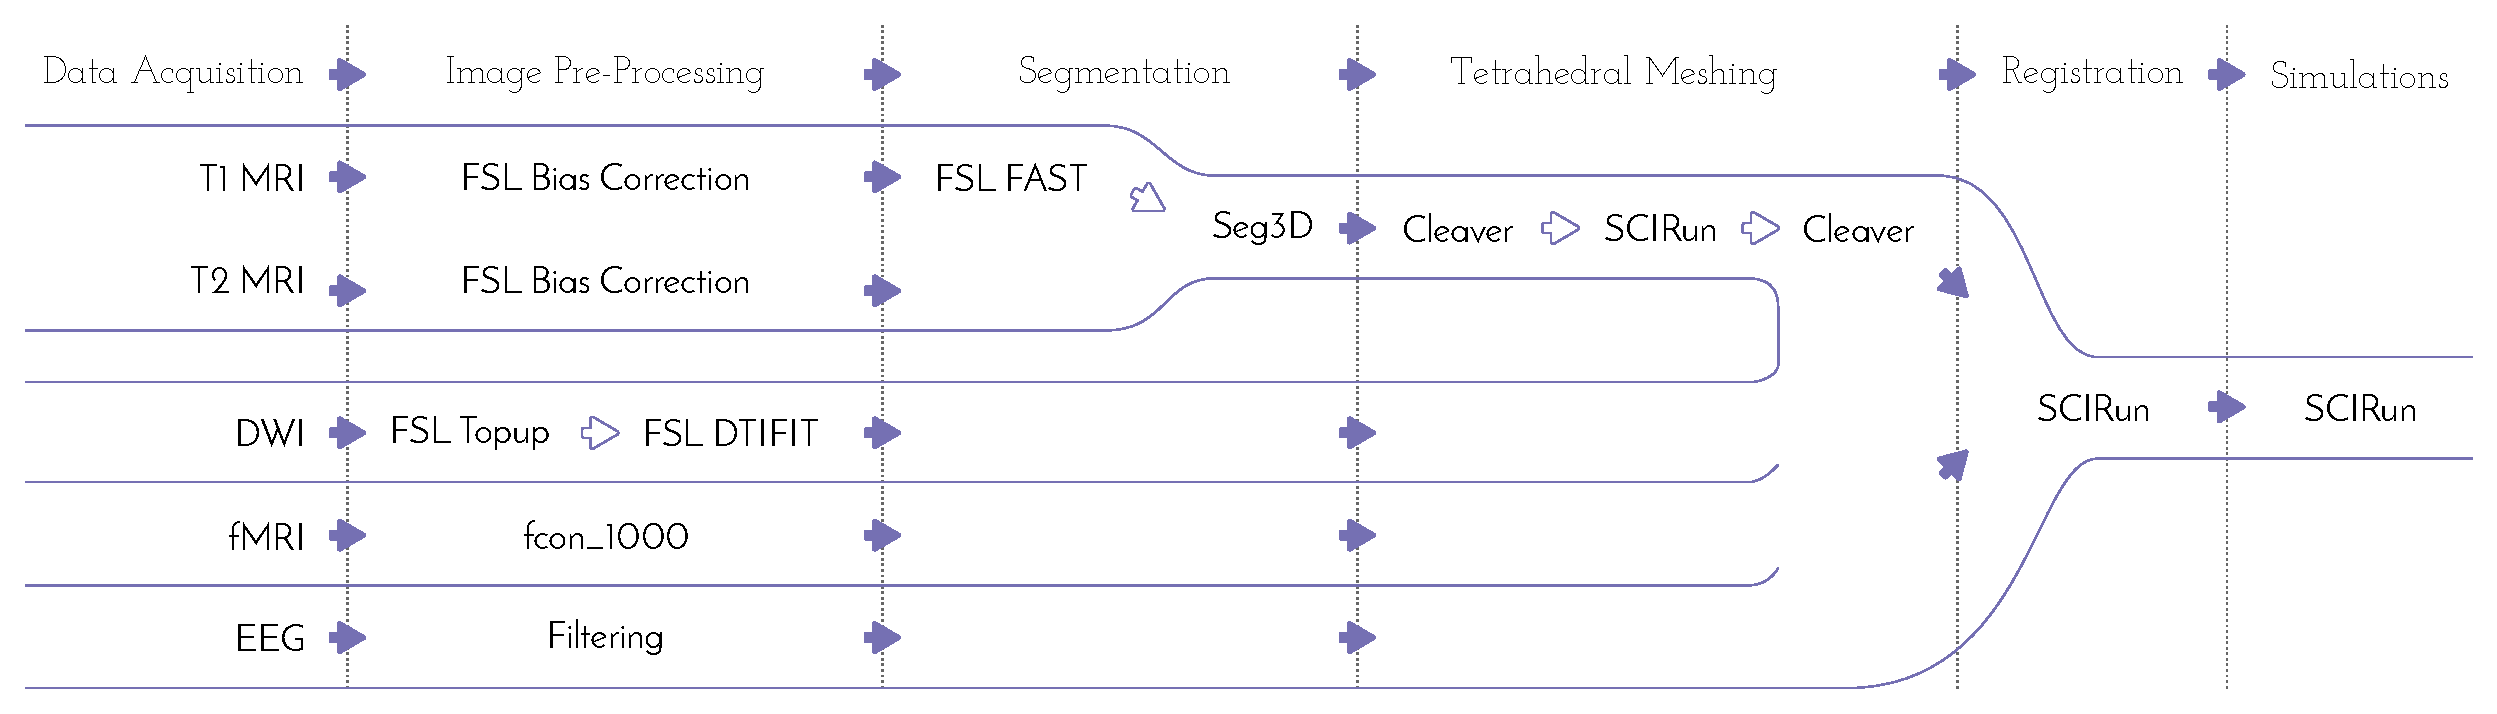
\includegraphics[width=\textwidth]{Figures/pipeline}
    \caption{Comprehensive head/brain model pipeline. Data sources are shown on the left with software packages used for creating the head/brain model in the middle and the simulation software on the right.}
    \label{fig:pipeline}
\end{figure}

\subsection{Data Acquisition}
\label{sec:Data}

%%% Image and EEG Acquisitions 

To construct a high-resolution, personalized, anisotropic volume conductor whole-head model, $T_1$-, $T_2$- weighted, diffusion-weighted, and functional magnetic resonance images (MRI) were acquired on a healthy female subject, 23 years of age, on a Skyra 3T full-body scanner (Siemens Medical Solutions, Erlangen, Germany).

The $T_1$-weighted scan was performed with a three-dimensional magnetization-prepared, rapid gradient echo (MPRAGE) sequence \cite{ref:mprage}. The parameters used were as follows: echo time: 3.41ms; repetition time: 2500ms; flip angle: 7 $^{\circ}$; resolution matrix size: 256x256 pixels; field of view: 256mm; 208 sagittal slices with a slice thickness of 1mm. Acquisition time was 10:42 minutes.

The $T_2$-weighted scan was performed with a SPACE (sampling perfection with application)-optimized contrast using different flip angle evolutions - sequence \cite{ref:space}. The parameters used were as follows: echo time: 406ms; repetition time: 3200ms; resolution matrix size: 256x256 pixels; field of view: 256mm; 208 sagittal slices with a slice thickness of 1mm. Acquisition time was 5:34 minutes.

The diffusion-weighted images (DWI) were acquired with multiband, two-dimensional, echo-planar imaging (EPI) \cite{ref:epi}. Both phase-encoding directions were performed (anterior to posterior (AP) and posterior to anterior (PA)) with 64 diffusion directions each. Further sequence parameters for each scan were as follows: echo time: 76.8ms; repetition time: 4070ms; flip angle: 90 $^{\circ}$; resolution matrix size: 104x104 pixels; field of view: 208mm; 60 slices with 2.5mm slice thickness. Acquisition time was 5:05 minutes each.

The functional MRI (fMRI) scans were acquired with a blood-oxygenation-level dependent contrast (BOLD) sequence. The following parameters were used: echo time: 76.8ms; repetition time: 780ms; flip angle: 55 $^{\circ}$; resolution matrix size: 104x104 pixels; field of view: 210mm; 72 slices with 2mm slice thickness. Acquisition time was 10:32 minutes.

Continuous electroencephalograms (EEGs) were recorded using a 128-channel and 256-channel HydroCel Geodesic Sensor Net that was connected to a NetAmps 400 amplifier and referenced online to a single vertex electrode. Channel impedances were kept at or below 50 kOhms, and signals were sampled at 250Hz. The EEGs were recorded while the subject sat quietly in a chair, alternating 2 minute epochs of eyes open and eyes closed, for a total of 12 minutes.

All acquisition reports are included with the dataset.

\subsection{Preprocessing of Images}
\label{sec:preprocess}

%FSL
\begin{wrapfigure}[14]{hr}{3cm}
    \centering
    \vspace{-63pt}
    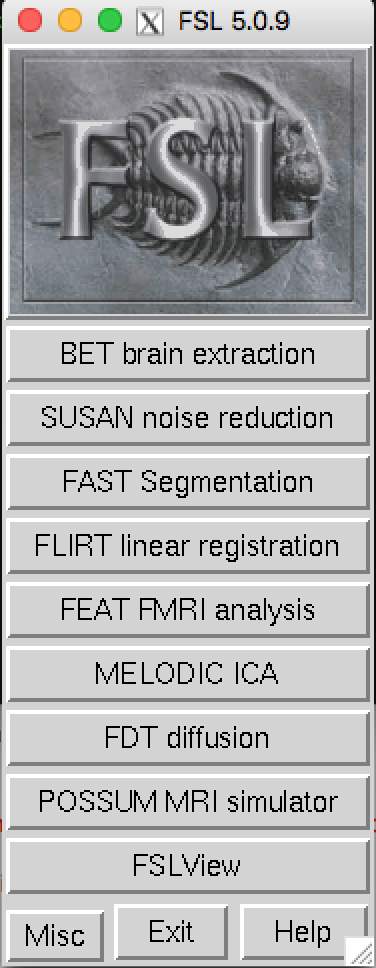
\includegraphics[width=3cm]{Figures/FSL}
    \caption{FMRIB software library user interface.}
    \label{fig:fsl}
\end{wrapfigure}

\subsubsection{MRI Correction}

A bias field signal is a low-frequency, smooth signal that corrupts MRI images due to inhomogeneities in the magnetic fields of the MRI machine by blurring images, thereby reducing the high frequencies of the images, such as edges and contours. The signal changes the intensity values of image pixels so that the same tissue has a different distribution of grayscale intensities across the image. \cite{ref:bias} We applied an estimated bias field correction on the $T_1$ and $T_2$ MRIs using FMRIB Software Library (FSL) FAST (Figure \ref{fig:fsl}) \cite{ref:fslfast}, which will be further described in Section \ref{sec:Seg}.

\subsubsection{DWI Distortion Correction}

DWIs performed with EPI sequences are prone to distortions from rapid switching of diffusion-weighting gradients, movement from the scanning table, and movement from the subject. The diffusion data were collected with reversed phase-encoded blips (AP and PA), resulting in pairs of images with distortions in opposite directions. From these pairs, we estimated the susceptibility-induced off-resonance field using a method \cite{ref:fsltopup1} similar to what is currently implemented in FSL.\cite{ref:fsltopup2} We then combined the two images into a single corrected image using FSL's topup and eddy command line tools. Details on this process are included in the Appendix in Section \ref{sec:distortion}.

\subsubsection{Diffusion Tensor Images}

After we preprocessed the DWI images, we calculated diffusion tensor images (DTI) using FSL's DTIFIT toolbox \cite{ref:dtifit} (Figure \ref{fig:dtifit}) and SCIRun \cite{ref:scirun}, a problem-solving environment for modeling, simulation, and visualization of scientific problems. We used the output from DTIFIT, the eigenvalues and eigenvectors of the DTI data, as input for a SCIRun network (Figure \ref{fig:maketensornet}) to build and visualize the conductivity tensor field. Details on using DTIFIT are included in the Appendix in Section \ref{sec:dtifit}.

\begin{figure}[H]
    \centering
    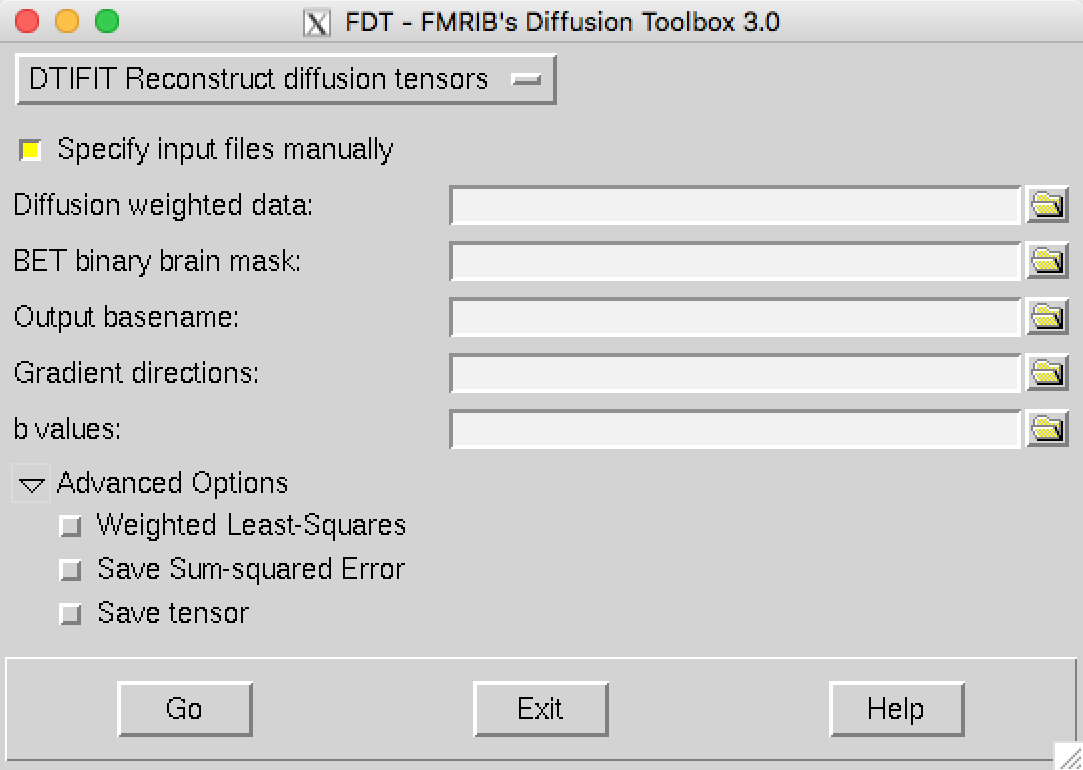
\includegraphics[width=.8\textwidth]{Figures/DTIFIT}
    \caption{FSL DTIFIT user interface.}
    \label{fig:dtifit}
\end{figure}

\subsubsection{fMRI}
\label{sec:fmripre}

We preprocessed the fMRI data using the 1000 Functional Connectomes (fcon) Project pipeline scripts \cite{ref:fcon}, which performed anatomical preprocessing, functional preprocessing, registration to the $T_1$ MRI, segmentation, and nuisance signal regress. The outline pipeline used on this fMRI dataset, specific to the University of Utah, can be found at \url{https://bitbucket.org/UtahBrainNetworks base_prep}, which includes instructions for installation, compilation, and usage. We then converted the preprocessed fMRI data from a four-dimensional to a two-dimensional dataset to be visualized in SCIRun (Figure \ref{fig:fmrivisnet}). Details on this data conversion are included in the Appendix in Section \ref{sec:nifti}. 

\subsubsection{EEG}

We applied a 60Hz notch filter and its harmonics \cite{ref:filter} to the EEG data to create an EEG data matrix. The rows of the matrix corresponded to the channels (electrodes) of the EEG net and the columns corresponded to the time step. We removed the last two rows of the EEG data matrix, because these were controls for the experiment, and several columns at the beginning and end of the matrix, because they corresponded to taking the EEG net on and off the subject's head. Details on building the EEG data matrix are included in the Appendix in Section \ref{ref:eegmatlab}. 

\subsubsection{Registration}
\label{sec:reg}

Since the subject did not move in between the $T_1$ and $T_2$ MRI, registration was not necessary before segmentation and mesh generation. We generated the tetrahedral mesh from the segmentation and registered the cortical surface mesh to the DTI coordinate space with a manual, rigid registration (Figure \ref{fig:dtireg} - \textit{(left)}). We included the registration transformation matrix to the DTI coordinate space in the dataset. 

Registration of the fMRI dataset required spatial preparation to ensure a more accurate rigid registration. For each fMRI time step, we mapped the corresponding vector of fMRI data onto a lattice volume, rotated the volume 180 degrees about the $z$-axis, smoothed it with a median filter, applied a threshold to it to remove noise, and clipped the brainstem. After we applied the rigid registration to the cortical surface mesh, we continued the registration manually to ensure the most accurate registration (Figure \ref{fig:dtireg} - \textit{(right)}). 

\begin{figure}[H]
\begin{center}
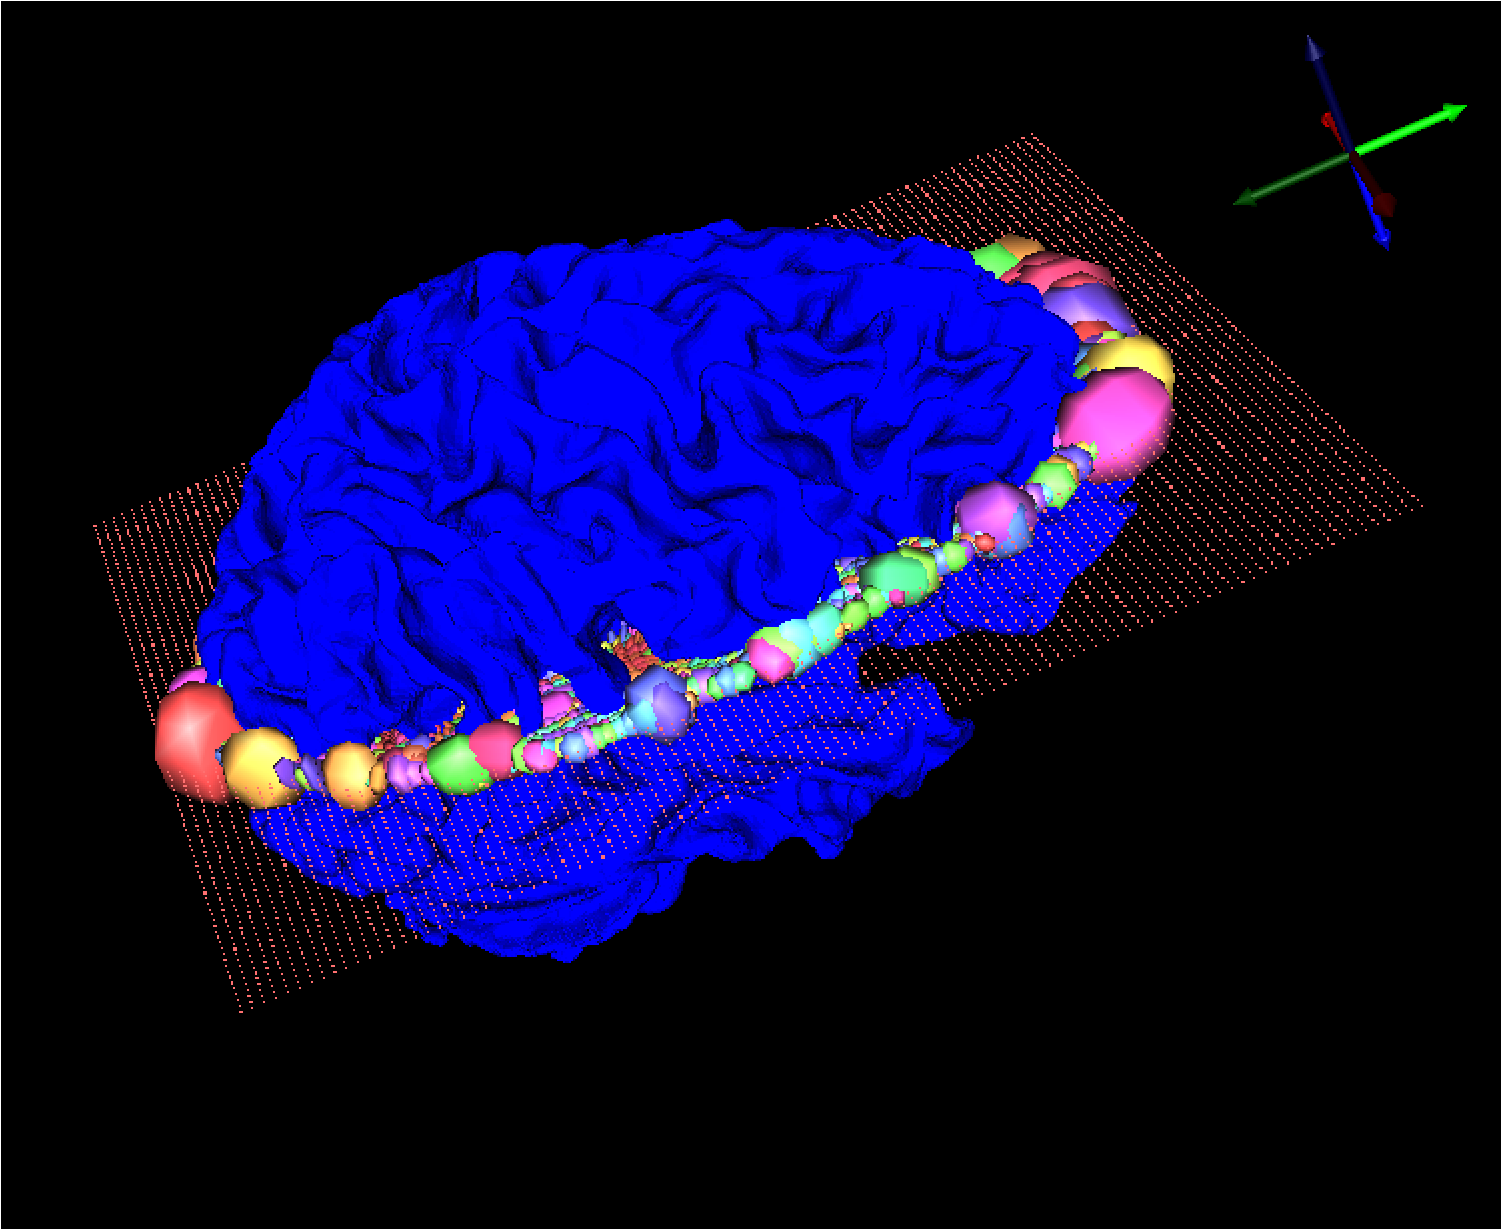
\includegraphics[height = 2.5in]{Figures/DTI_reg}
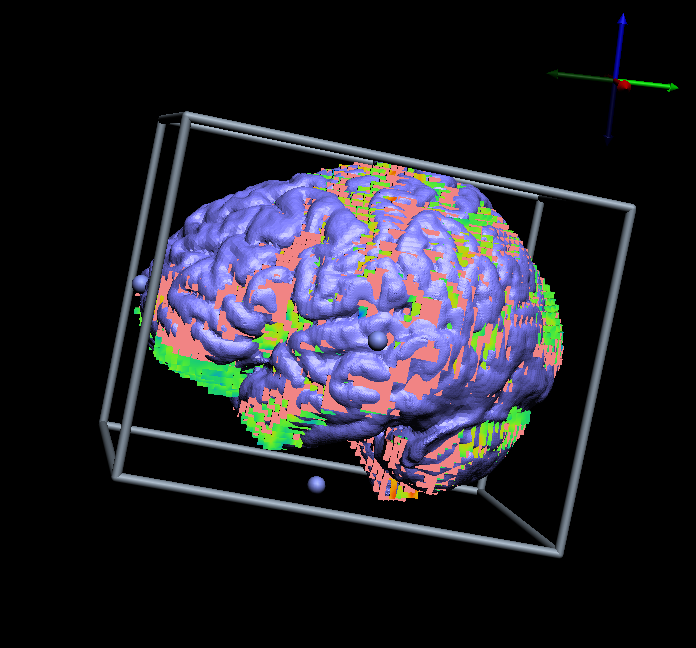
\includegraphics[height = 2.5in]{Figures/fmri_reg}
\caption{SCIRun manual registrations: cortical surface mesh to DTI registration \textit{(left)}, fMRI to cortical surface mesh registration \textit{(right)}.}
\label{fig:dtireg}
\end{center}
\end{figure}

The EEG geometry data from the ESI system consisted of dipole source locations (4800) and electrode locations (128 or 256). To register the electrode positions to the head mesh, we rotated them 180 degrees about the $z$-axis, applied a rigid registration, and projected the points onto the head surface mesh (Figure \ref{fig:eegreg}). We then applied a rigid registration to register the dipoles to the cortical surface mesh.

\begin{figure}[H]
\begin{center}
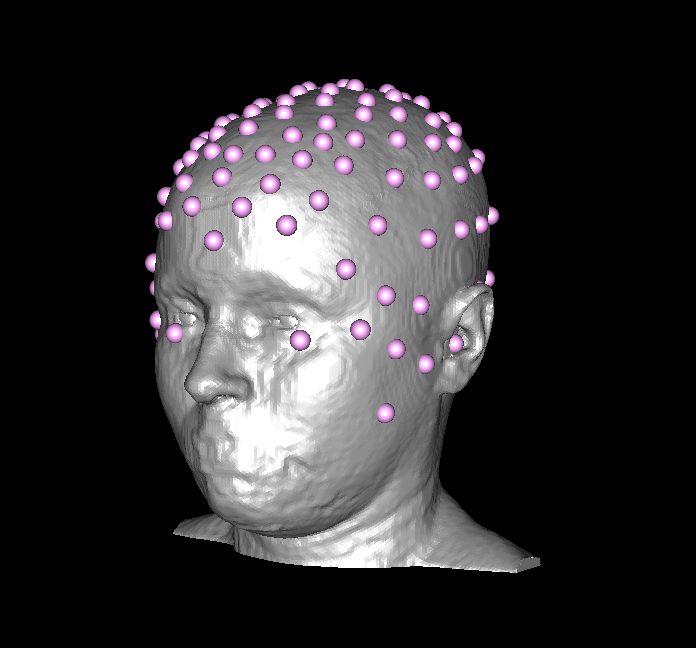
\includegraphics[height = 2.84in]{Figures/128_eeg_reg}
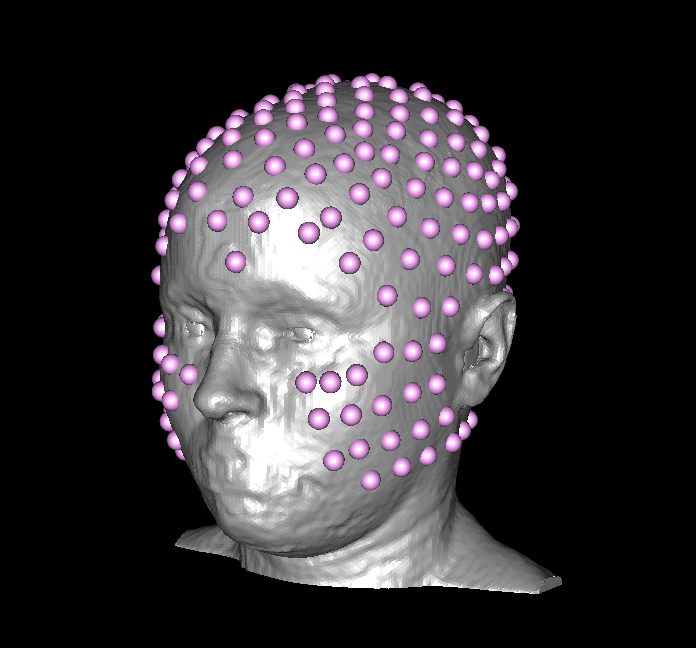
\includegraphics[height = 2.84in]{Figures/256_eeg_reg}
\caption{SCIRun manual registration of physical electrodes to head surface mesh: 128 electrodes \textit{(left)}, 256 electrodes \textit{(right)}.}
\label{fig:eegreg}
\end{center}
\end{figure}

The SCIRun networks for registration are included in the Appendix in Section \ref{sec:networks} in Figures \ref{fig:isofornet} - \ref{fig:eegvisnet}.

\subsection{MRI Segmentation of Tissues}
\label{sec:Seg}

%%% Preparation for segmentation, trials, manual work 

We segmented the head volume using FSL and Seg3D, a free volume segmentation and processing tool, \cite{ref:seg3d} into air, cerebral spinal fluid (CSF), white matter, gray matter, skull, sinus, eyes, and scalp. We used FSL for initial segmentation and Seg3D for all further segmentation, including thresholding and manual editing.

We generated the initial brain segmentation with FSL from the $T_1$ MRI by stripping the skull with the brain extraction tool (BET) \cite{ref:bet1} (Figure \ref{fig:bet2}) and then segmenting with FAST segmentation (Figure \ref{fig:fslfast}). FSL FAST outputs grayscale probability images of CSF, white matter, and gray matter layers (Figure \ref{fig:fastout}) as well as a bias-corrected $T_1$ MRI (Figure \ref{fig:fastoutbias}). 

\begin{figure}[H]
\begin{center}
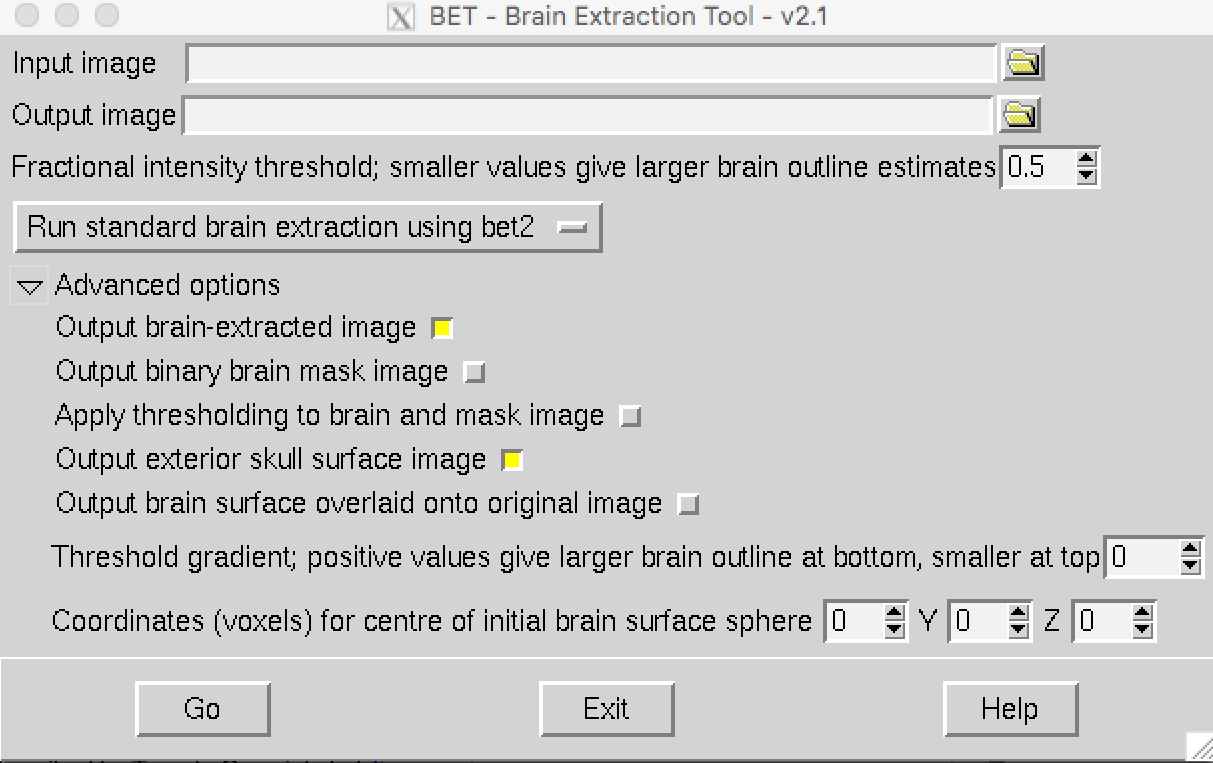
\includegraphics[width=.8\textwidth]{Figures/BET2}
\caption{FSL's BET2 tool.}
\label{fig:bet2}
\end{center}
\end{figure}

\begin{figure}[H]
    \centering
    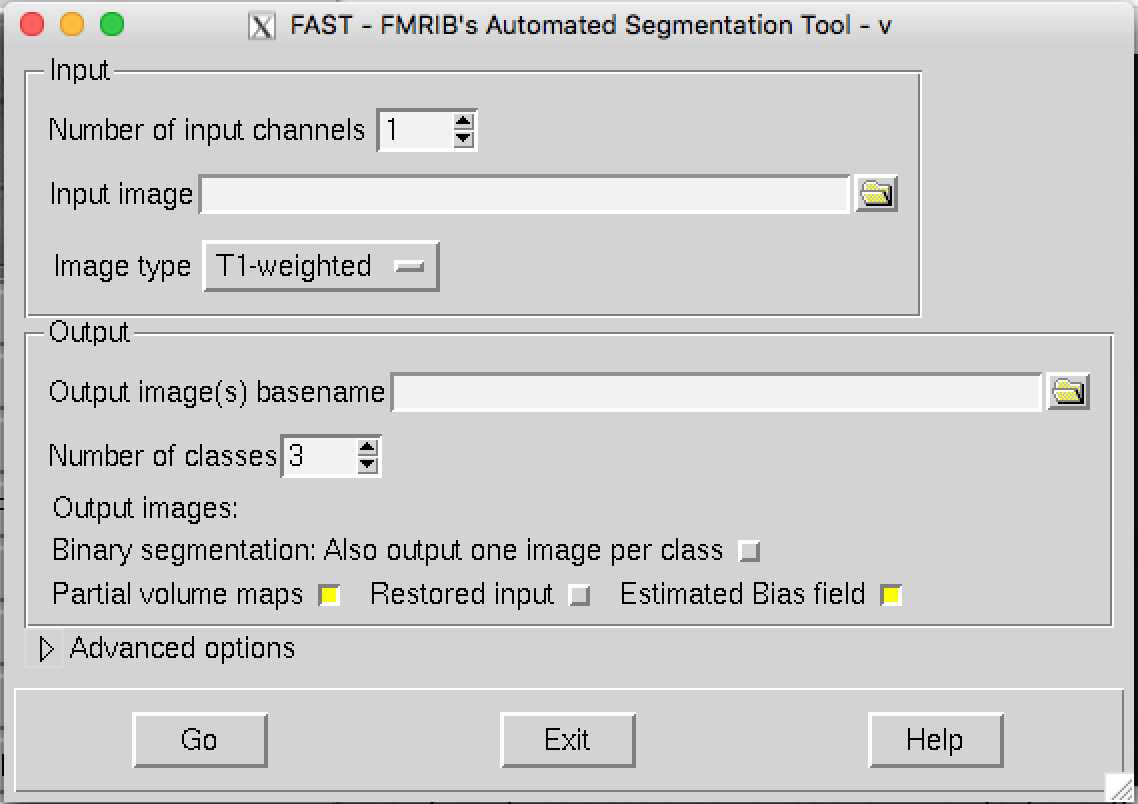
\includegraphics[width=.8\textwidth]{Figures/FSL_FAST}
    \caption{FSL FAST user interface.}
    \label{fig:fslfast}
\end{figure}

\begin{figure}[H]
\begin{center}
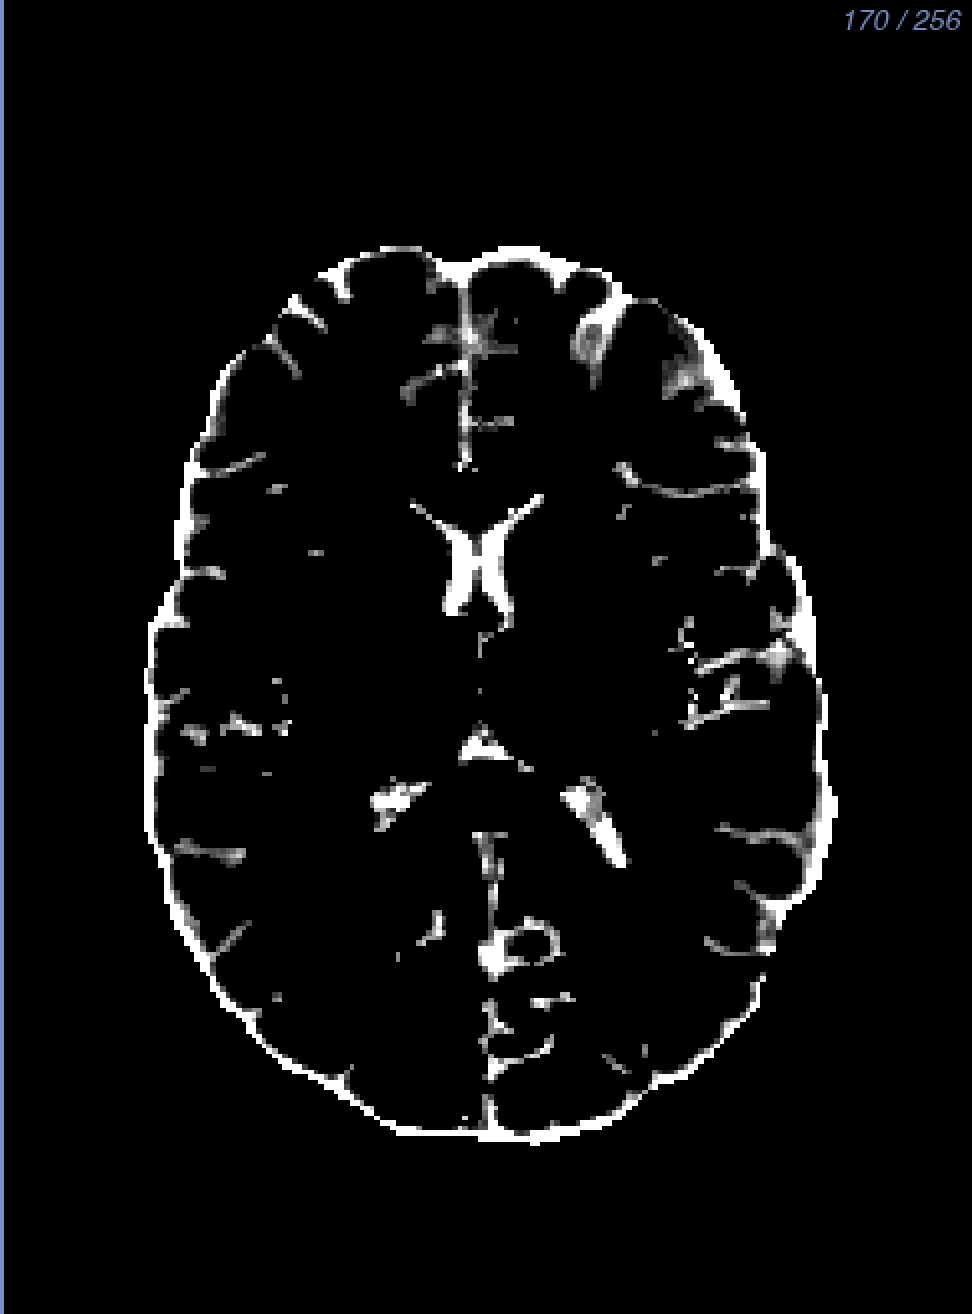
\includegraphics[width=.32\textwidth]{Figures/FSLFAST_csf}
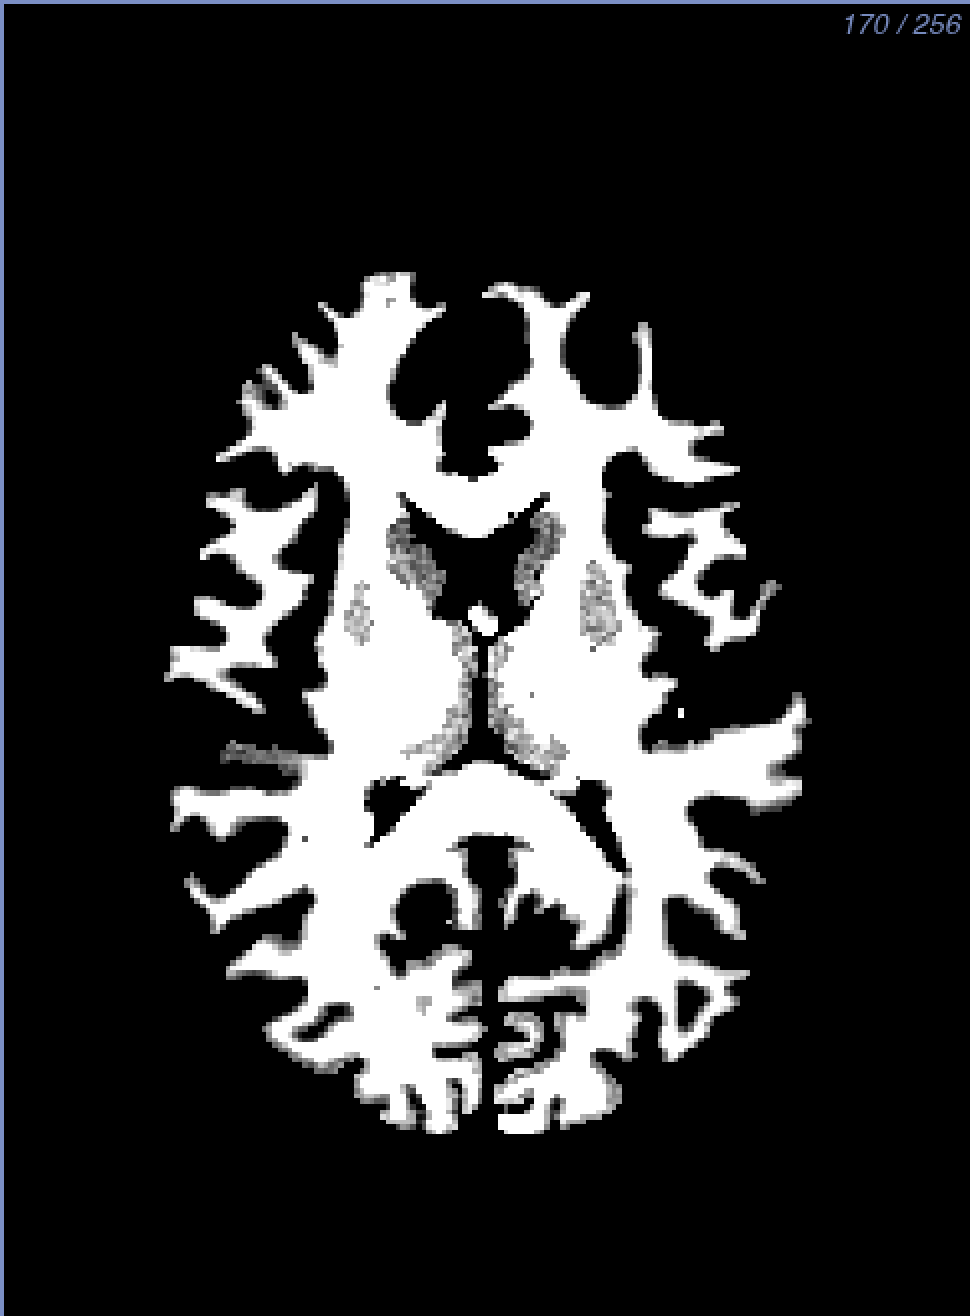
\includegraphics[width=.32\textwidth]{Figures/FSLFAST_wm}
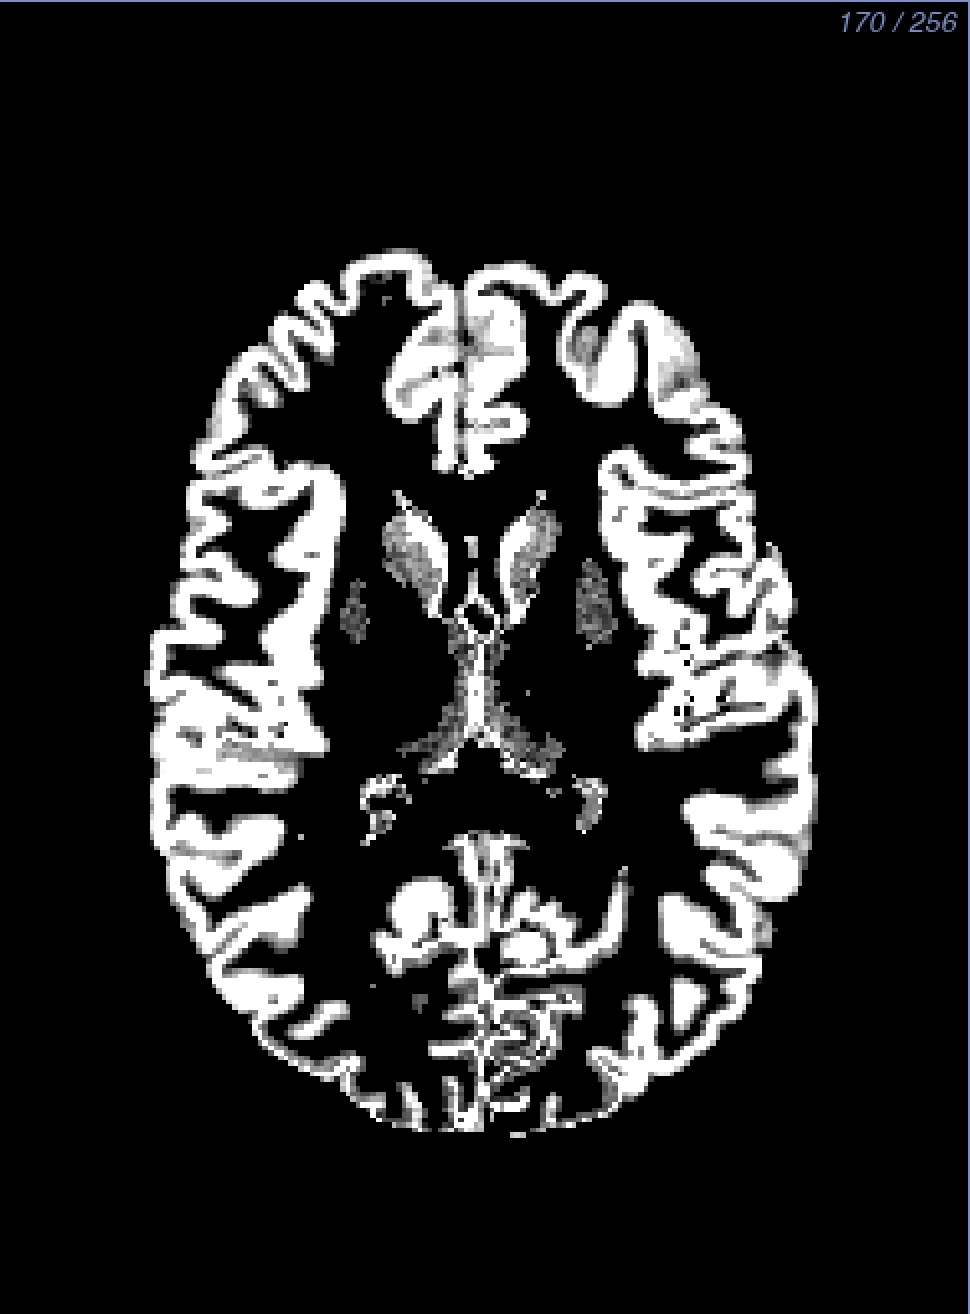
\includegraphics[width=.32\textwidth]{Figures/FSLFAST_gm}
\caption{FSL FAST output: CSF \textit{(left)}, white matter \textit{(center)}, gray matter \textit{(right)}.}
\label{fig:fastout}
\end{center}
\end{figure}

\begin{figure}[H]
\begin{center}
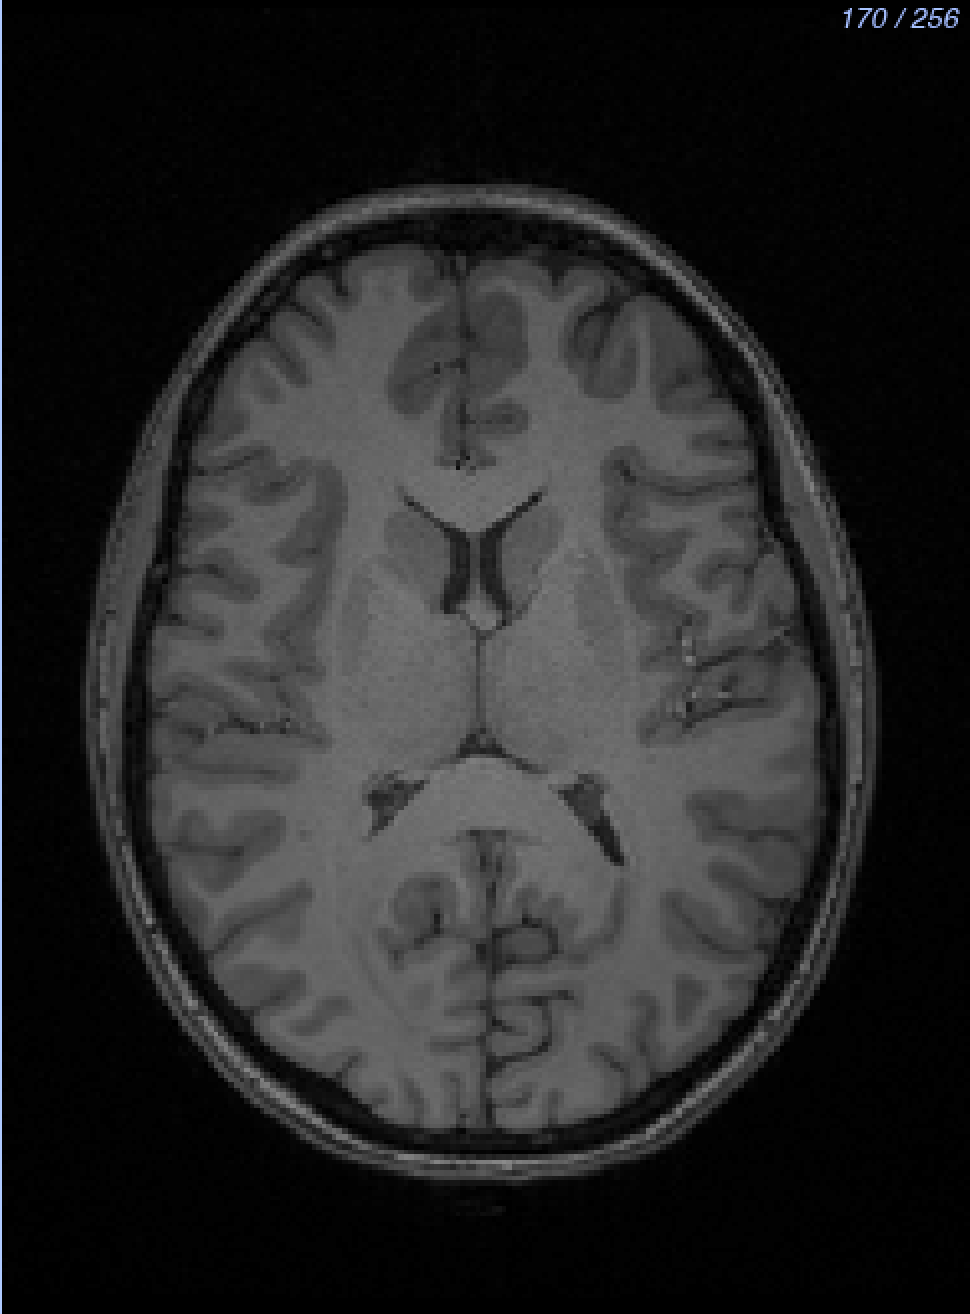
\includegraphics[width=.45\textwidth]{Figures/Original_T1}
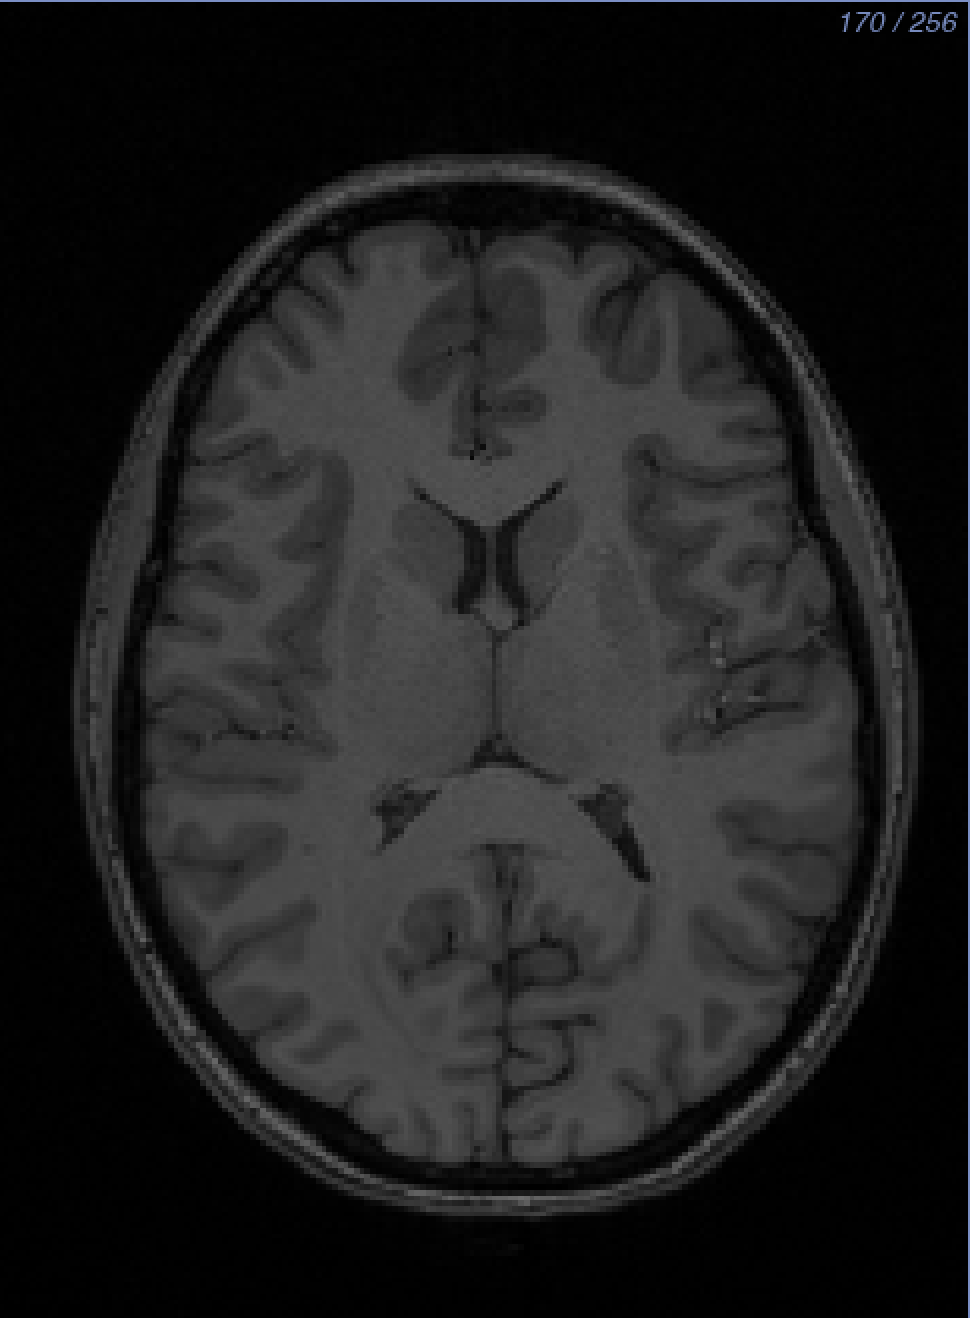
\includegraphics[width=.45\textwidth]{Figures/T1_corrected}
\caption{FSL FAST output: $T_1$ MRI image before bias correction \textit{(left)} and after bias correction \textit{(right)}.}
\label{fig:fastoutbias}
\end{center}
\end{figure}


We created segmentations from the FSL FAST output by thresholding the probability images and by inspecting and manually editing each slice to remove any crossover between the layers, to add more detail, and to smooth out noisy areas. We started with the white matter layer because it is the innermost layer (Figure \ref{fig:wm}).

\begin{figure}[H]
\begin{center}
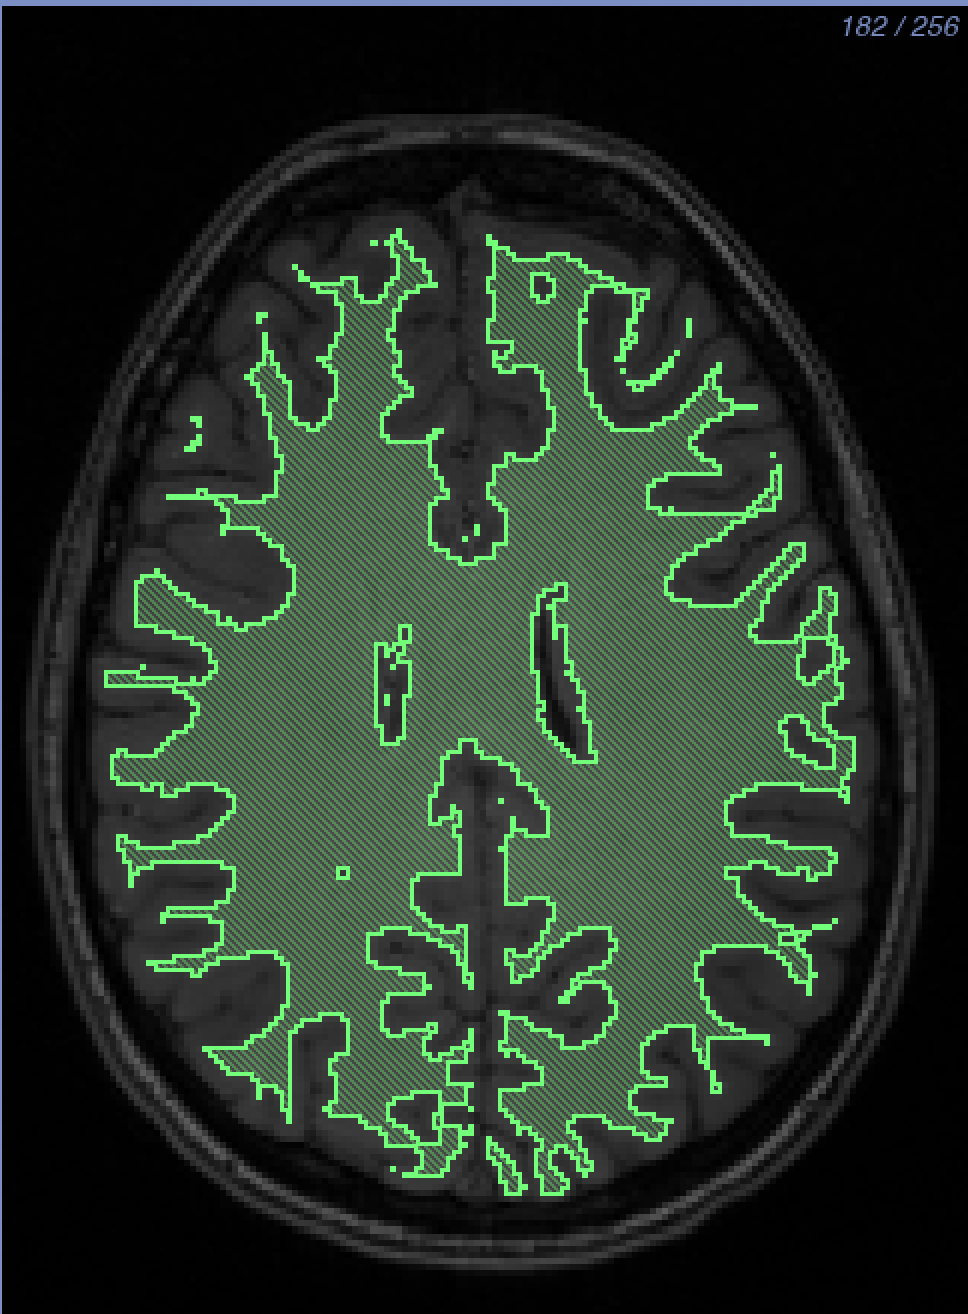
\includegraphics[width=.49\textwidth]{Figures/whitematter_before}
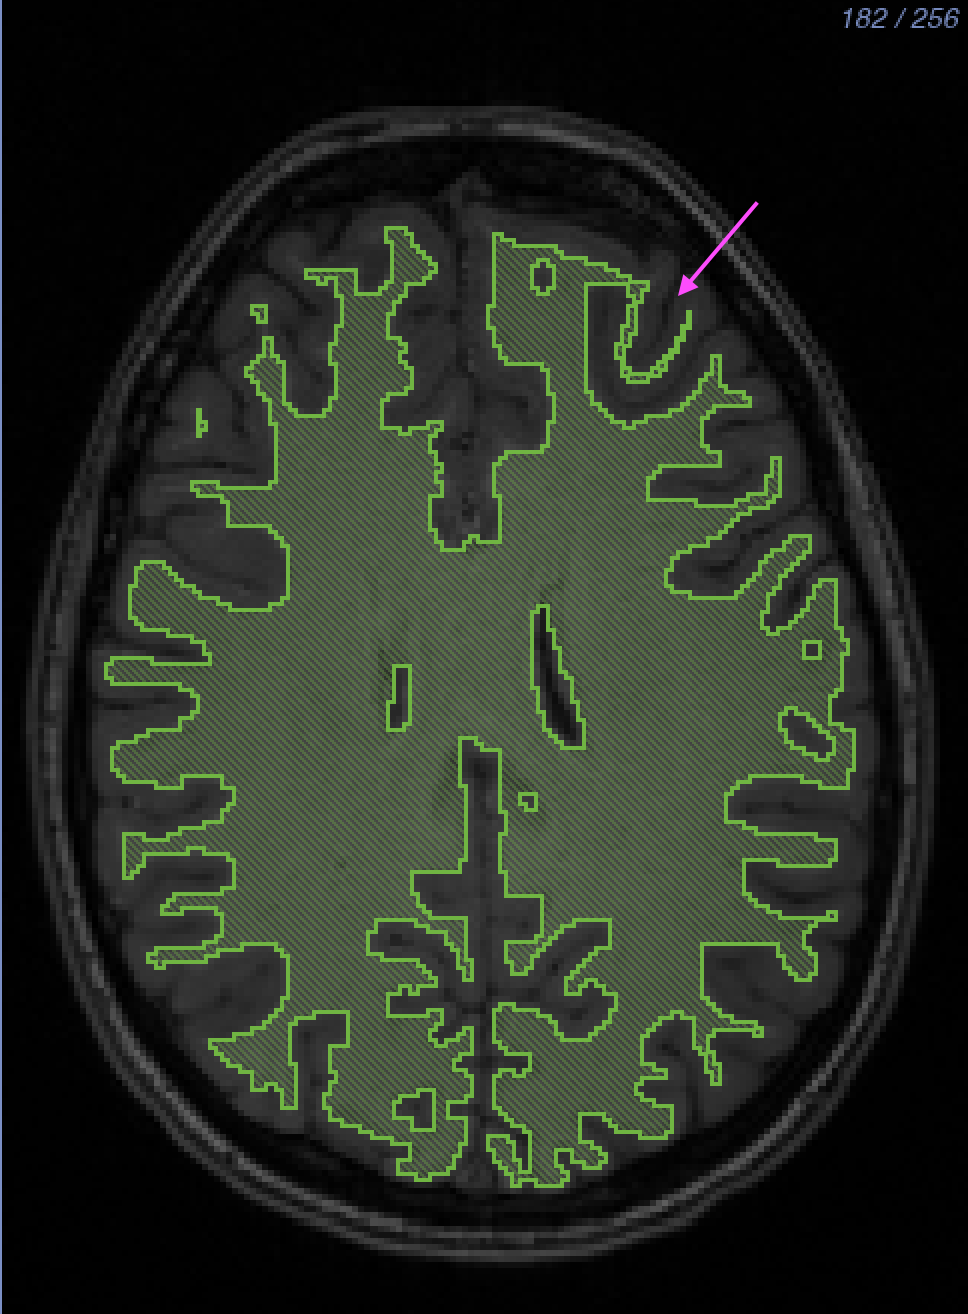
\includegraphics[width=.49\textwidth]{Figures/whitematter_after}
\caption{White matter segmentation: Before \textit{(left)} and after \textit{(right)} manual segmentation. The hook feature in the upper right-hand corner is a notable change between the two layers. The layer is more full and has less noise.}
\label{fig:wm}
\end{center}
\end{figure}

After we segmented the white matter, we created a threshold layer from the FSL FAST output for the gray matter. We then inspected and manually edited each slice in every direction. After manual editing, we removed the white matter layer from the gray matter using a Boolean remove mask filter to ensure no overlap between the layers. Lastly, we added a gray matter nuclei segmentation to the gray matter layer. The thresholding algorithms in Seg3D produced noise around these nuclei because of their grayscale similarities to white matter. To fix this noise, we segmented the nuclei area manually using the paintbrush tool in Seg3D. We added the nuclei to the gray matter layer using a Boolean OR mask filter, and removed any overlap from the white matter layer using a Boolean remove mask filter. We manually filled any holes between the two layers that could be assigned to either white or gray matter layers (Figure \ref{fig:gm}).

\begin{figure}[H]
\begin{center}
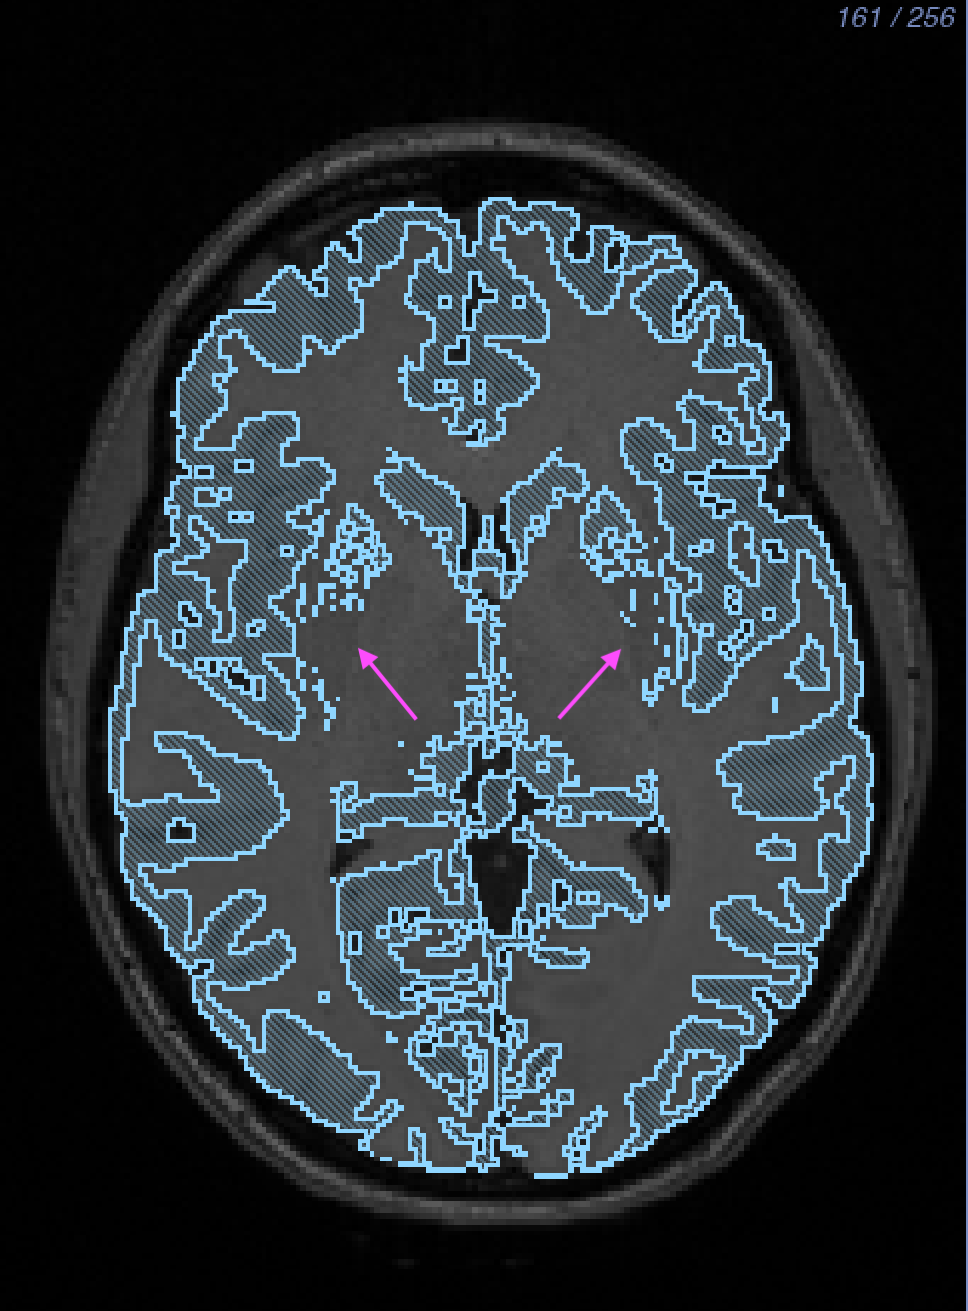
\includegraphics[width=.49\textwidth]{Figures/greymatter_before_nuclei}
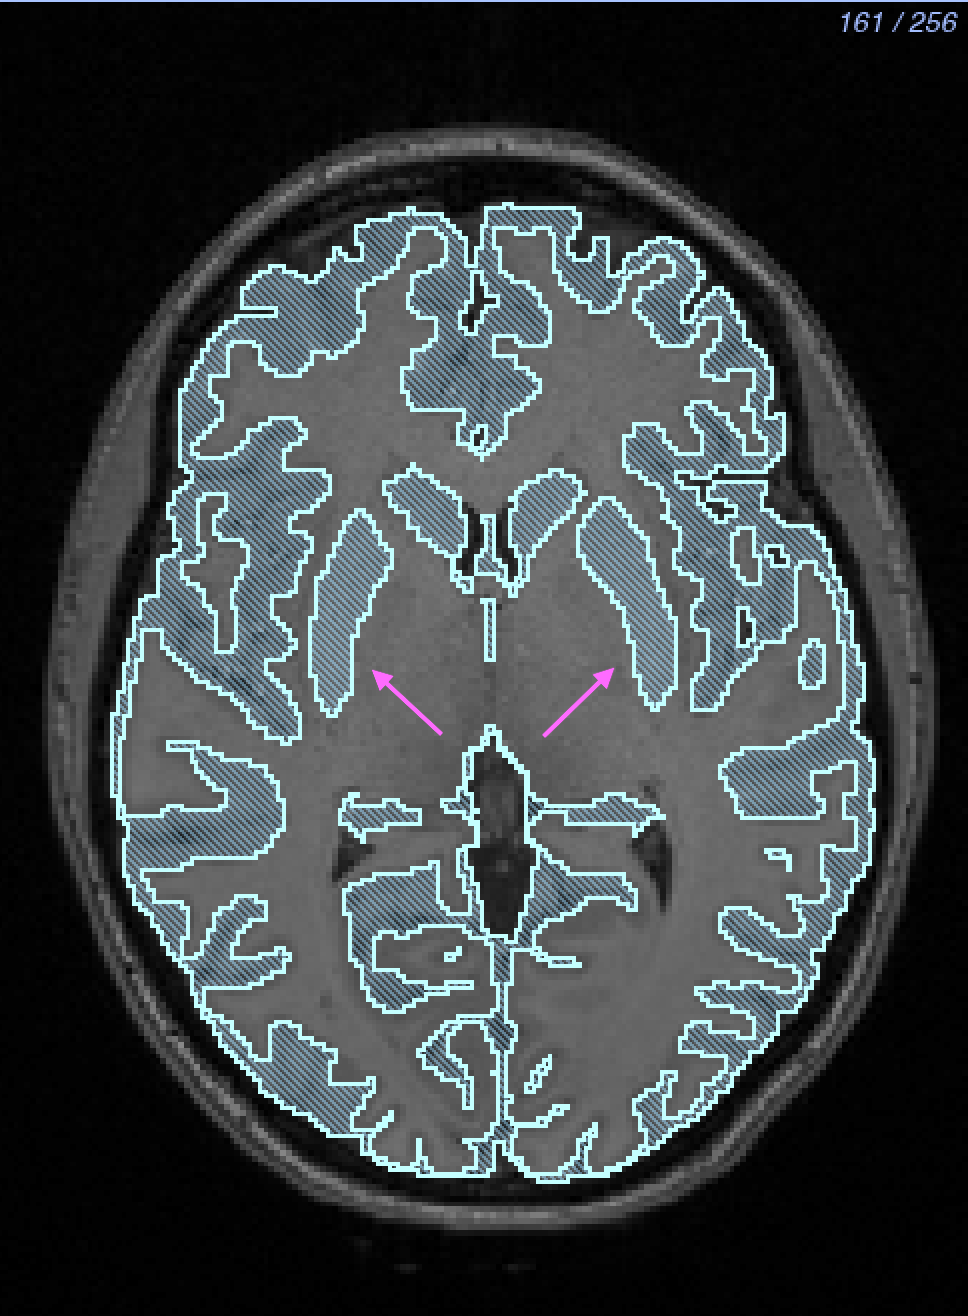
\includegraphics[width=.49\textwidth]{Figures/greymatter_added_nuclei}
\caption{Gray matter segmentation: Before \textit{(left)} and after \textit{(right)} manual segmentation. Gray matter nuclei located in the center of the brain were segmented manually.}
\label{fig:gm}
\end{center}
\end{figure}

After we completed the segmentation of gray and white matter, we segmented CSF by creating a solid threshold layer for the entire brain and removing the white and gray matter layers using a Boolean remove mask filter (Figure \ref{fig:csf}). We then checked the white matter, gray matter, and CSF layers for holes, both on the surface and inside the segmentation between layers. We also performed a manual quality check on the layers to ensure that they were at least two pixels wide throughout. This thickness criterion helped to ensure a quality tetrahedral mesh.

\begin{figure}[H]
\begin{center}
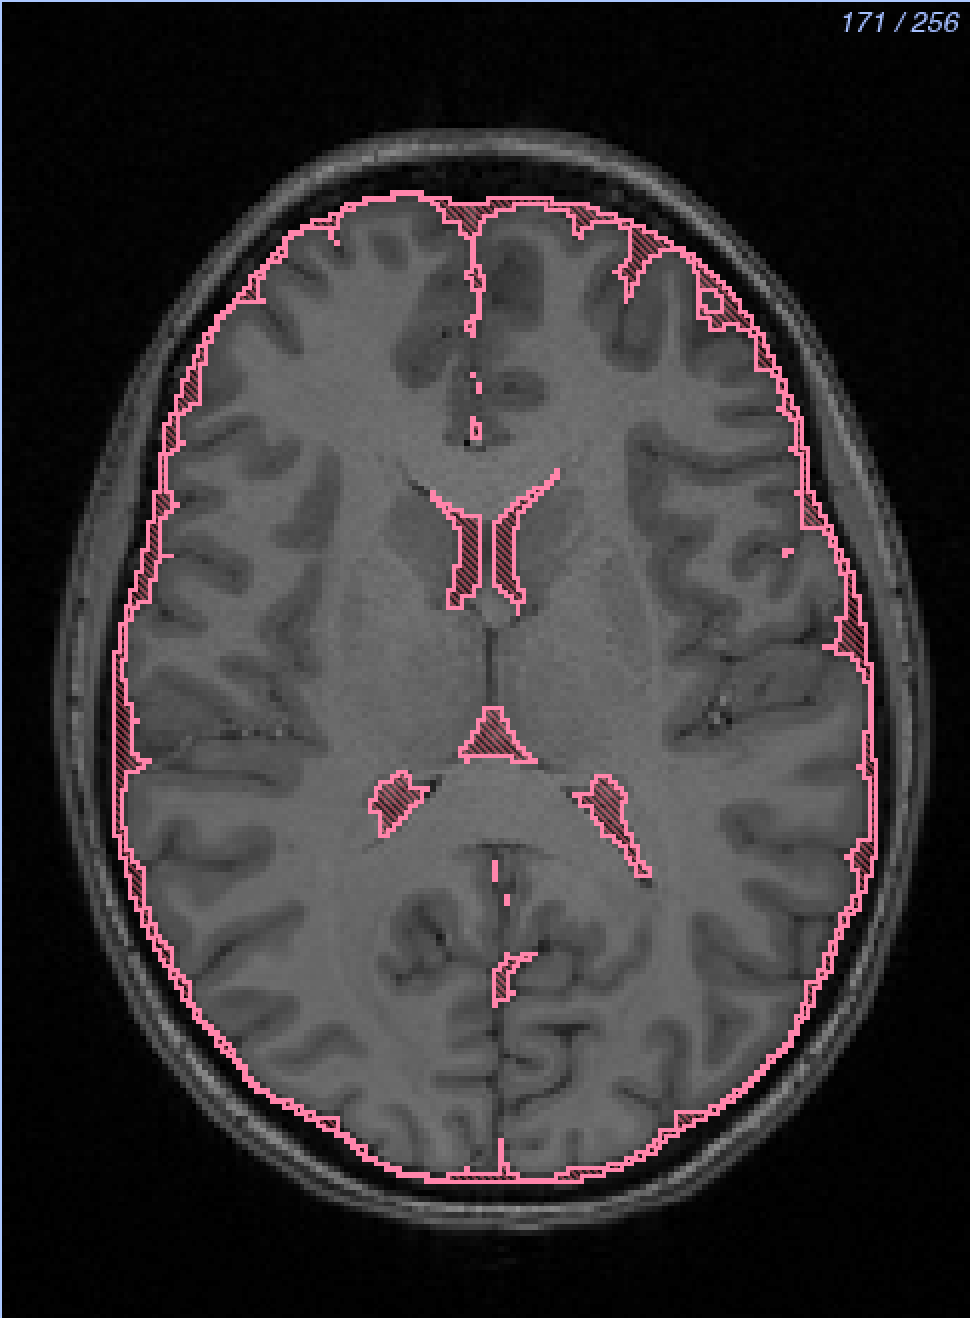
\includegraphics[width=.49\textwidth]{Figures/CSF_seg}
\caption{CSF segmentation.}
\label{fig:csf}
\end{center}
\end{figure}

We segmented the skull and sinus from an MR-based synthetic pseudo-CT image (Figure \ref{fig:skull}-\textit{(left)}). We used an improved iterative version of the patch-based method, as described by Torrado-Carvajal et al., \cite{ref:pseudoct} that takes the $T_1$ and $T_2$ images as input and synthesizes the pseudo-CT based on both images, providing more refined and accurate bone boundaries.

For the skull segmentation, we applied a median filter with a one-pixel radius to the pseudo-CT image and thresholded the white pixels. We then manually edited each slice in every direction to add detail and to smooth noise (Figure \ref{fig:skull}-\textit{(center)}). Since the subject had a permanent dental retainer that caused white pixels throughout her mouth in the Pseudo-CT image, we segmented the mouth as solid bone. We deemed acceptable because the EEG cap used did not cover the subject's mouth. 

For the internal air segmentation, including the sinuses, esophagus, and ear canals, we thresholded the black pixels of the pseudo-CT image and manually edited each slice in every direction (Figure \ref{fig:skull}-\textit{(right)}). We also performed a quality check on both layers to ensure they did not contain holes or have any layer overlap and were at least two pixels thick.

\begin{figure}[H]
\begin{center}
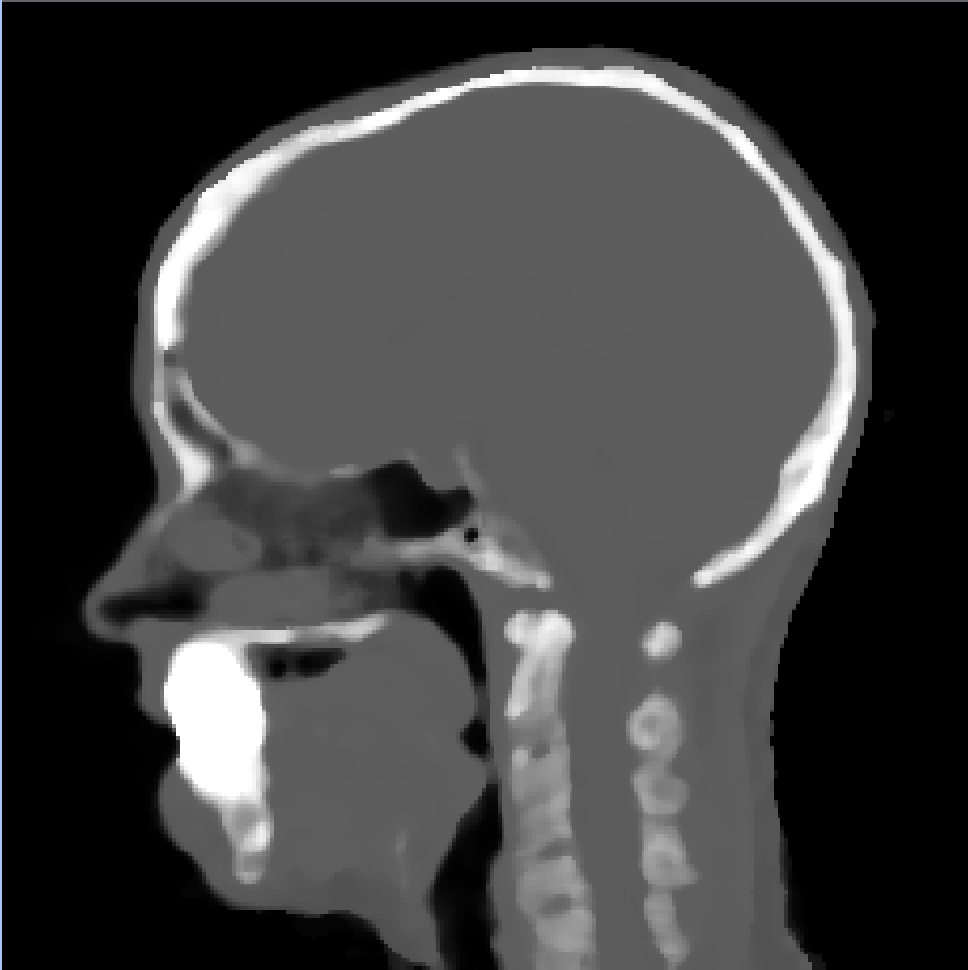
\includegraphics[width=.32\textwidth]{Figures/pseudo_CT}
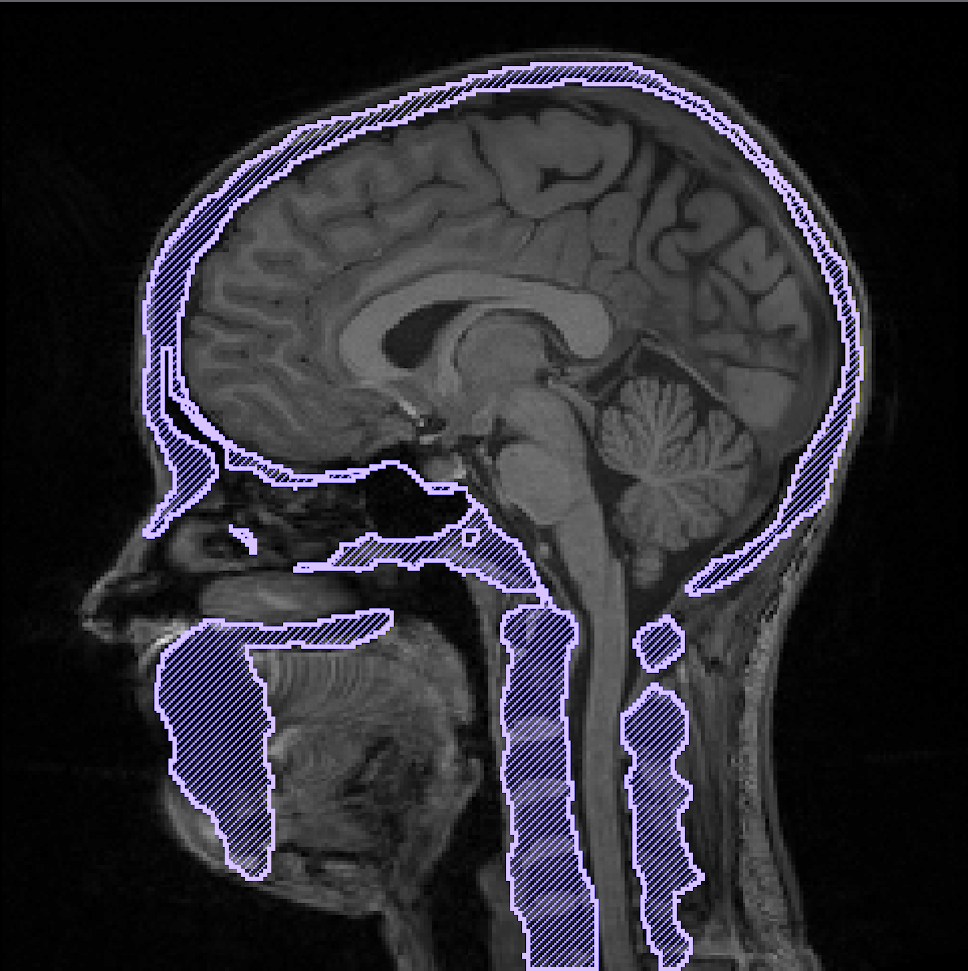
\includegraphics[width=.32\textwidth]{Figures/skull_seg}
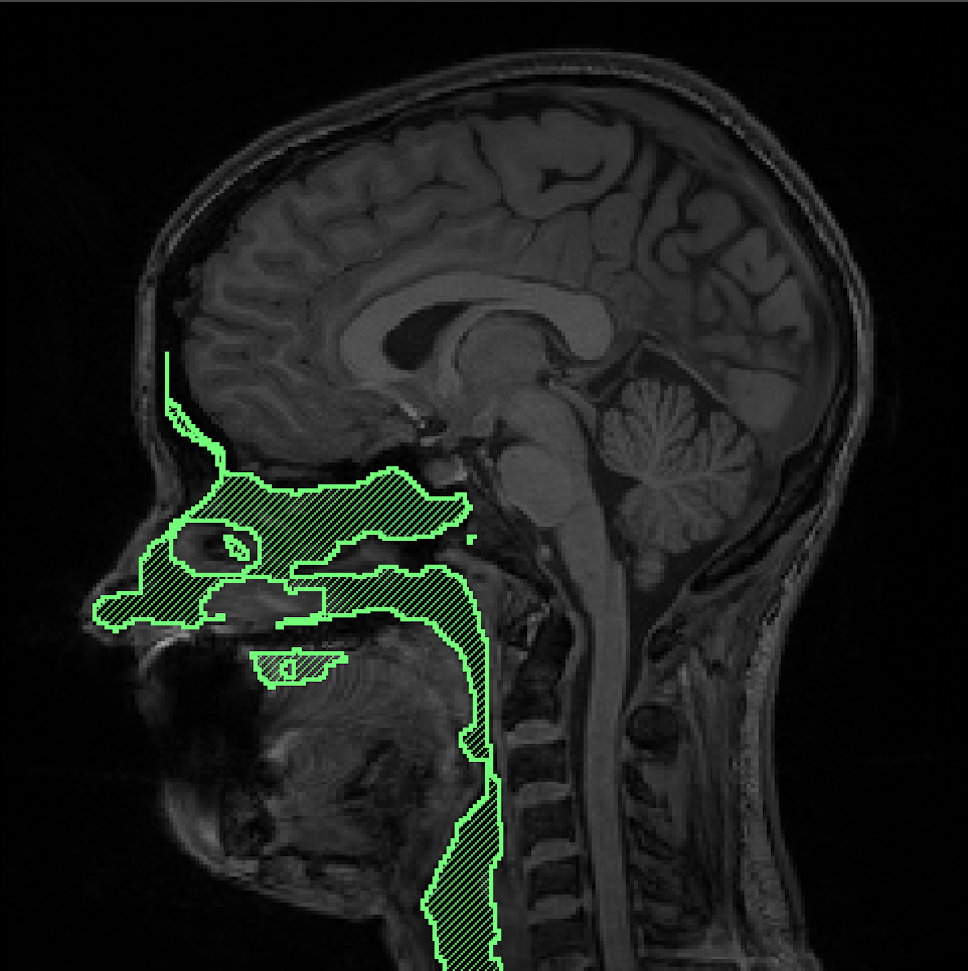
\includegraphics[width=.32\textwidth]{Figures/sinus_seg}
\caption{Skull segmentation: Pseudo-CT image \textit{(left)}, skull layer \textit{(center)}, and sinus layer \textit{(right)}.}
\label{fig:skull}
\end{center}
\end{figure}

We then segmented the eyes, skin, and external air. We segmented the eyes by thresholding the $T_2$ MRI, and the skin layer by thresholding the entire head volume and removing all previous segmentation layers using a Boolean remove mask filter. We performed a quality check on the skin layer to ensure that it was at least two pixels thick. The areas that required significant correction were the bridge of the nose, the bottom of the chin, and the sides of the head. Finally, we included pixels not previously assigned as the external air layer. We checked the entire segmentation to make sure there were no holes between layers to assure a quality mesh and accurate simulation results. 

\begin{figure}[H]
\begin{center}
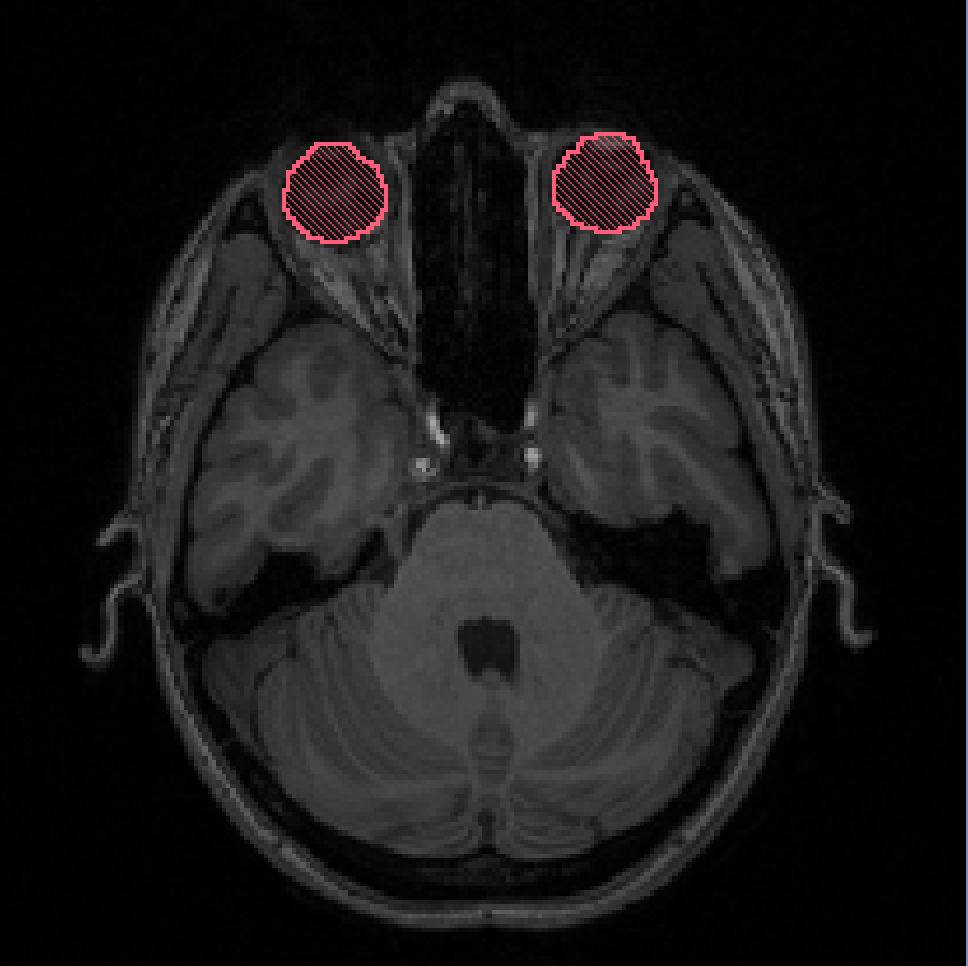
\includegraphics[width=.32\textwidth]{Figures/eyes_seg}
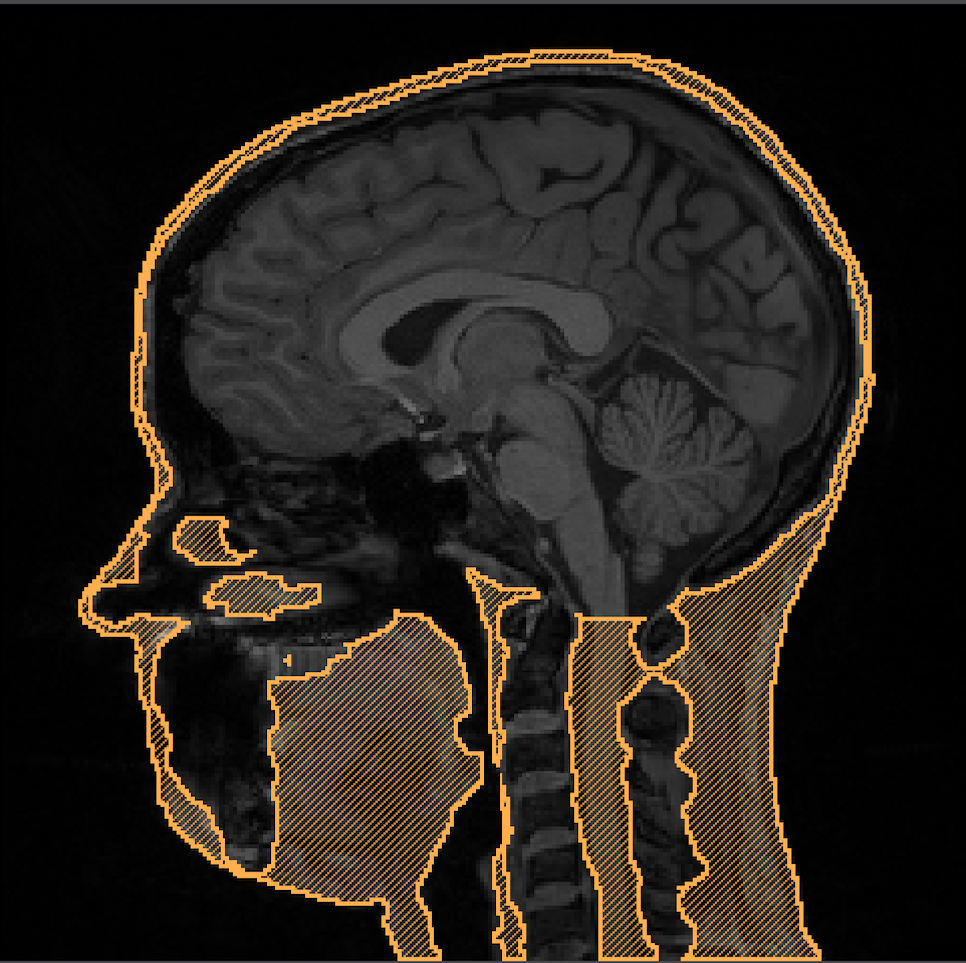
\includegraphics[width=.32\textwidth]{Figures/skin_seg}
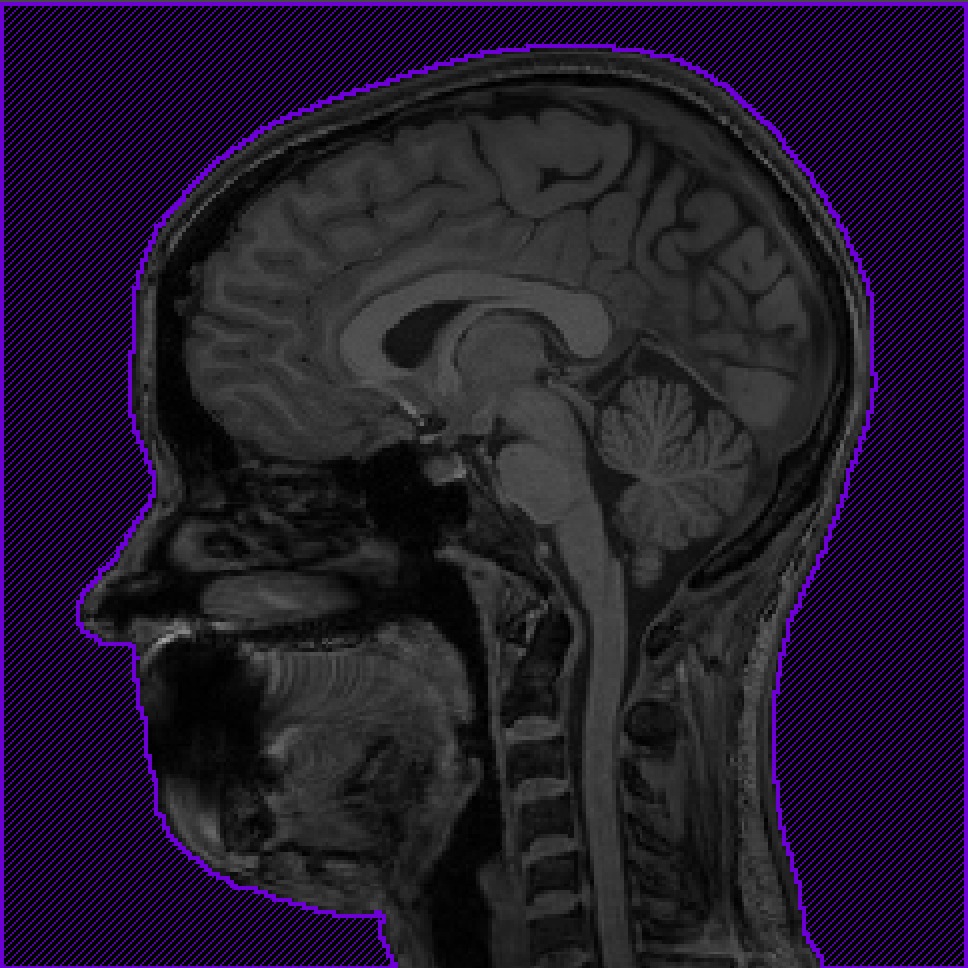
\includegraphics[width=.32\textwidth]{Figures/air_seg}
\caption{Eye segmentation with $T_2$ MRI \textit{(left)}, skin segmentation \textit{(center)}, and air segmentation \textit{(right)}.}
\label{fig:skull}
\end{center}
\end{figure}

The segmentation of the image data took approximately 100 hours, most of which was dedicated to manual editing. A breakdown of time per segmentation layer is shown in Table \ref{tab:seg}.

\begin{table}[H]
\centering
\caption{Segmentation Time}
\label{tab:seg}
\begin{tabular}{|c|c|}
\hline
Segmented Tissue    & Amount of Work (hrs) \\ \hline
White Matter       & 40                   \\ \hline
Gray Matter         & 20                   \\ \hline
CSF                 & 4                    \\ \hline
Skull and Sinus     & 35                   \\ \hline
Eyes, Scalp, \& Air & 8                    \\ \hline
\end{tabular}
\end{table}

\subsection{Mesh Generation}
\label{sec:mesh}

%%% Settings for mesh generation, issues 

We used our full-head segmentation to generate realistic three-dimensional geometries for use in subsequent finite element simulations. We generated a smooth, linear, subject-specific, boundary-conforming, quality, high-resolution, tetrahedral mesh using the Cleaver software \cite{ref:cleaver} on a Late 2013 Mac Pro with a 2.7 Ghz 12 Core Intel Xeon E5 processor with 64 GB of RAM and an AMD FirePro graphics card using the parameters listed in Table \ref{tab:cleaver}. Cleaver is a multimaterial meshing package that produces structured meshes of tetrahedral elements with guaranteed minimum element angles, resulting in quality meshes that require fewer computational resources. 

\begin{table}[H]
\centering
\caption{Clever Settings (High Resolution)}
\label{tab:cleaver}
\begin{tabular}{|c|c|}
\hline
scaling factor                    & 0.6                 \\ \hline
size multiplier                   & 1.0                 \\ \hline
lipschitz                         & 0.2                 \\ \hline
padding                           & 0                   \\ \hline
element sizing method             & adaptive            \\ \hline
\end{tabular}
\end{table}

We created indicator functions, which describe the location of the surface with subgrid accuracy, by calculating inverted distance maps of each layer in the full-head segmentation in Seg3D using the distance map filter. To reduce the size of the mesh, we generated a new mesh, changing only the scaling factor parameter to 1.0 from the parameters in Table \ref{tab:cleaver}. We exported the computing sizing field from Cleaver and manipulated it in SCIRun by changing how quickly the elements increased in size. We input the changed sizing field into Cleaver with the same indicator functions and successfully cleaved a new, smaller, quality mesh. Both sizing fields are included in the dataset.

\subsection{Mathematical Modeling}
\label{sec:math}

%%%MATH

The forward and inverse EEG problems are governed by a generalized Poisson equation (\ref{eq:1}). We used the head mesh, with associated inhomogeneous and anisotropic conductivity regions, as a volume conductor to solve the following boundary value problem:
%
\begin{equation}
\label{eq:1} \nabla\cdot\sigma\nabla\Phi = -I_{V} \;\;\;\;\mbox{ in
}\Omega,
\end{equation} 
%
where $\Phi$ is the electrostatic potential, $\sigma$ is the electrical conductivity tensor, and $I_{V}$ is the current per unit volume defined within the solution domain, $\Omega$. For the forward EEG problem, we solved equation \ref{eq:1} for $\Phi$ with a known description of $I_{V}$ and the Neumann boundary condition:
%
\begin{equation} \sigma\nabla\Phi\cdot{\bf
n} = 0\;\;\;\;\;\mbox{ on }\Gamma_{H}, 
\end{equation} 
%
which says that the normal component of the electric field is zero on the surface interfacing with air (here denoted by $\Gamma_{H}$). For testing purposes, we used dipoles for the current source. We calculated the electrical and potential fields everywhere within the head model. \cite{SCI:Joh2015c}

\subsubsection{Electrical Conductivity Preparation}
\label{sec:cond}

All electrical conductivities were homogeneous for each tissue with the exception of the white matter when using DTI data. The isotropic conductivities \cite{ref:cond} we used are shown in Table \ref{tab:cond}.

\begin{table}[H]
\centering
\caption{Isotropic Tissue Conductivity}
\label{tab:cond}
\begin{tabular}{|c|c|}
\hline
Tissue Type               & Isotropic Conductivity $(S/m)$ \\ \hline
\hline
White Matter              & 0.1429                         \\ \hline
Gray Matter               & 0.3333                         \\ \hline
Cerebrospinal Fluid (CSF) & 1.79                           \\ \hline
Skull                     & 0.001                          \\ \hline
Skin                      & 0.4346                         \\ \hline
Sinus                     & 1e-6                           \\ \hline
Eyes                      & 0.5051                         \\ \hline
\end{tabular}
\end{table}

When we added the DTI tensor data, we used two approaches to convert the tensor data to conductivities. The first was scaling the data \cite{ref:scaling}: 

\begin{equation}
\label{eq:scaling}
\sigma_{aniso} = \frac{\sigma_{iso}}{\sqrt[3]{d_1d_2d_3}}D,
\end{equation}
where $D$ is the diffusion data, $d_i$ is the $i$th eigenvalue of $D$, and $\sigma_{iso}$ is the white matter isotropic conductivity. The second method gave the white matter a fixed ratio of conductivity:

\begin{equation}
\label{eq:fixed}
\sigma_{aniso} = \begin{bmatrix}
v_1\\
v_2\\
v_3\\
W\\
\end{bmatrix}, 
W = \begin{bmatrix}
\sigma_{iso}\\
\frac{\sigma_{iso}}{10}\\
\frac{\sigma_{iso}}{10}\\
\end{bmatrix},
\end{equation}
where $v_i$ is the $i$th eigenvector of $D$, $W$ is the white matter ratio vector, and the ratio is $10:1$.

We implemented both methods into the SCIRun networks for anisotropic forward problems (Figure \ref{fig:anisofornet}). 

\subsubsection{Numerical Methods}
\label{sec:numerical}

%%% This paragraph addresses Finite Element Discretization

We computed solutions to equation \ref{eq:1} using the finite element method. By applying Green's theorem to equation \ref{eq:1}, we generated the following weak formulation:
\begin{equation}
\label{eq:weakGreens}
\langle \sigma \nabla \phi, \nabla \bar{\phi} \rangle = -\langle I_v, \bar{\phi} \rangle
\end{equation}
where $ \bar{\phi}$ is an arbitrary test function, which can be thought of physically as a virtual potential field. By applying the Galerkin approximation to equation \ref{eq:weakGreens}, we can represent the finite element approximation as
\begin{equation}
\label{eq:galerkin}
\sum_{i = 0}^{N} \varepsilon_i \langle \sigma_{ij} \nabla \psi_{i}, \nabla \psi_{j} \rangle = -\langle I_v, \psi_i \rangle \quad j = 0, \dots, N,
\end{equation}
subject to the Dirichlet boundary condition. The finite element approximation of equation \ref{eq:1} can equivalently be expressed as a system of $N$ equations with $N$ unknowns $\varepsilon_i \dots \varepsilon_N$ (e.g., the electrostatic potentials). In matrix form, the above system can be written as $A \varepsilon = b$,  where $A=(a_{ij})$ is called the global stiffness matrix and has elements $(a_{ij}) = (\sigma_{ij} \nabla \psi_{i}, \nabla \psi_{j})$, and $b_i = -(I_v, \psi_i)$ is usually termed the load vector. For volume conductor problems, $A$ contains all the geometry and conductivity information of the model. \cite{SCI:Joh2015c}

%%% This paragraph addresses SCIRun as a solver
We used SCIRun to apply parameters and to solve equation \ref{eq:galerkin} numerically using linear basis functions for tetrahedral elements. Within the SCIRun environment, we applied isotropic and anisotropic conductivity tensors to the tetrahedral mesh as well as to inhomogeneous regions. We applied Dirichlet and Neumann boundary conditions to compute potentials using a conjugate gradient method with a Jacobi preconditioner (Figures \ref{fig:isofornet} - \ref{fig:anisofornet}).

\subsection{Simulations and Visualizations}
\label{sec:sim}

We performed all simulations and visualizations in SCIRun. All networks are shown in the Appendix in Section \ref{sec:networks} - Figures \ref{fig:maketensornet} - \ref{fig:eegvisnet}.

\subsubsection{Forward Problem}

Solving systems from a known source to the EEG electrodes, described in Section 2.5, is known as a forward problem. The opposite action, solving systems from the EEG data to a unknown source, is an inverse problem.  In this project, we built SCIRun example networks to solve forward problems with known sources and to write a lead field matrix for use in future inverse problems. We solved forward problems with isotropic and anisotropic conductivities, using DTI data for the direction of anisotropic conductivities.

The required inputs for the isotropic example network were the tetrahedral head mesh, isotropic conductivities, the head segmentation, the physical electrode locations, and dipole sources. The SCIRun network allowed the user to choose a dipole as a current source from the set for a forward simulation. The network also removed fiducial electrodes from the dataset. We registered the mesh to the head segmentation using the rigid registration previously described in Section \ref{sec:reg}. We then registered the electrodes and the dipoles to the mesh coordinate space, as described in Section \ref{sec:reg}. After we removed any flat tetrahedra from the mesh, we mapped the conductivities to their respective tissues. We solved the system with the mapped data and the chosen dipole sources. We then extracted the solution onto the head surface and the electrode locations for visualization. We also used streamlines and isopotential lines for visualization.

For the anisotropic example, the network was similar to the isotropic example with the exception of the scaled diffusion tensor data used as conductivities for white matter, and the DTI to mesh transform as additional input. We registered the head mesh, electrodes, and dipoles to the DTI space with a rigid registration, as described in Section \ref{sec:reg}; the head segmentation was not needed.

\subsubsection{fMRI}

We visualized the fMRI data one time step at a time using the two-dimensional matrix, described in Section \ref{sec:fmripre}, as input by extracting one column at a time. We registered the fMRI to the tetrahedral mesh as described in Section \ref{sec:reg}. After registration, we mapped the smoothed fMRI data onto the mesh using a mapping matrix with a linear interpolation basis.

\subsubsection{EEG}

We visualized EEG data on the physical electrode locations, which we registered to the head mesh with a rigid registration, as described in Section \ref{sec:reg}, after removing the fiducials from the electrode dataset. We obtained the filtered EEG data one time step at a time by extracting the column of the matrix. We then placed the electrodes onto the mesh and mapped the EEG data onto the electrodes. An example EEG network is shown in Figure \ref{fig:eegvisnet}. Each EEG electrode configuration has its own SCIRun network.

